\documentclass[11pt]{article}
\usepackage{amssymb}
\usepackage[fleqn]{amsmath}
\usepackage{semantic}
\usepackage{listings}
\usepackage{hyperref}
\usepackage{graphicx}
\usepackage{algpseudocode}


\title{Evolution of ORM Systems: Formal Foundations}
\author{Ondrej Macek}

\begin{document}

\maketitle
\begin{abstract}
The evolution of a software is a common issue during software lifecycle. The evolution od code and database are usually separated tasks. We discuss the evolution of software in context of  software created using an object oriented programming language and a relational database. The formal definition of the evolutionary framework is introduced in this paper. Special attention is given to the data stored in databases (instances) and theirs consistency during evolution process.
\end{abstract}

\textbf{Keywords:} data evolution, data migration
\section{Introduction}
The evolution of a software is a common issue during software development. The evolution can occur from many reasons in different stages of software lifecycle. The evolution of a software created using an object oriented programming language and a relational database is usually processed in two steps - as a code refactoring and as a database migration, which is processed as an SQL script. The code refactoring is supported by many IDEs, whereas the database migration is usually processed manually. There are frameworks and tools capable of database evolution, nevertheless these tools are usually not capable to solve complicated migration cases or preserve stored data. Another disadvantage of such an approach to data evolution is the evolution has to be define twice - as a code refactoring and as a database migration.

There are three main goals of our evolutionary framework: 1) provide one source of evolution definition for both: code and database 2) provide a tool, which will be able to preserve stored data and information.

This paper provides a formal definition of such a framework, which is based on model driven architecture. There are defined models representing an application and database in this paper, together with transformations which are able to perform an evolution of the whole software and preserve data.



The paper is organized as follows: in Section \ref{sec:evoIntro} the concept of ORM software and its evolution is discussed, then models of application and database are introduced in Section \ref{sec:appModel} and in Section \ref{sec:dbModel}, the ORM is defined in Section \ref{sec:orm} and the evolutionary transformations are defined in Section \ref{sec:Evolutionaty-Transformations}.

\subsection{Note on Used Notation}
Before the definition of the software is provided, the notation of function transcription has to be introduced. Usually the definition of a function consists of two parts - an effect of the function and conditions when the effect occurs. We decide to use bit different transcription to simplify the notation and to improve understanding of functions, instead of usually used:
\begin{align*}
& f(x) = effect \; if \; condition 
\end{align*}
we use following notation:
\begin{align*}
& f(x) =   \inference{condition}{effect}
\end{align*}

\section{ORM Software}
\label{sec:evoIntro}
\begin{figure}
\centering
	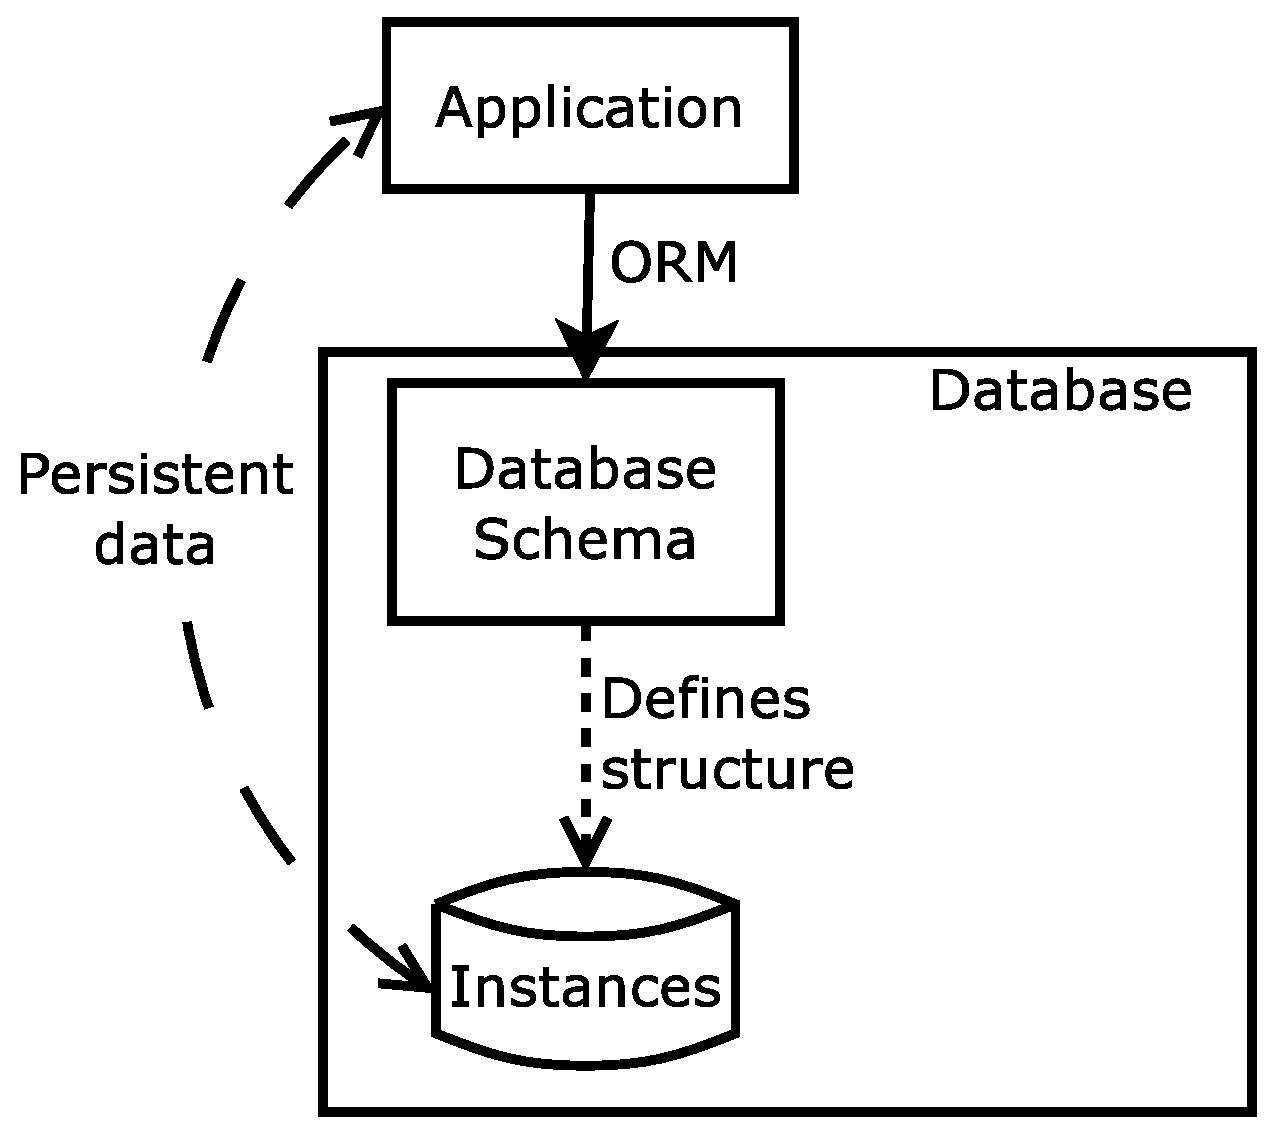
\includegraphics[scale=0.3]{./images/system}
	\caption{The model of one generation of an ORM system consists of application persistent layer and relational database for storing instances.}
\label{fig:appStructure}
\end{figure}
A software implemented using an object-oriented language, which uses relational database as a data storage (as illustrated in the Figure \ref{fig:appStructure}) is object of interest of this paper. There are three important components of such a software: application (its persistent layer concretely), database (consisting of database schema and stored data) and an ORM (we will use $\rho$ as a symbol for ORM), therefore we define a software as a triple consisting of an application and a database which are connected together by an ORM:
\begin{align*}
& \mathbf{software} = ( Application, Database, \rho )\\
& \mathbf{sw} : Application \times Database \times ORM \rightarrow  Software \\ 
\\
& \mathbf{application} \in Software \rightarrow Application \\
& application(sw(a, d, \rho)) = a \\ \\
& \mathbf{database} \in Software \rightarrow Database \\
& database(sw(a, d, \rho)) = d \\\\
& a \in Application, d \in Database
\end{align*}

The software has to be in consistent state so its users could have benefit from its usage. The state of the software is defined to communicate the sate of the software to its user, the symbol $\perp$ is used as a notation for inconsistent state. The components of a software (application and database) are transformed likewise, thus the state is defined for them too.
\begin{align*}
& 	\mathbf{state} = Consistent\; s \: | \: \perp,  \\\\
& 	s \in State \vee s \in Application \vee s \in Database
\end{align*}


%The function querying the state (it means consistency) of a software is defined as:
%\begin{align*}
%& 	\mathbf{consistent} : State \rightarrow Boolean \\
%& 	consistent(state(s)) = \begin{cases}
% 		\inference{s = Consistent \; s}{true}\\\\
% 		\inference{s = \perp}{false}\\
% \end{cases}\\
%& s \in Software
%\end{align*}
The consistency of application and database is discussed later in this paper. The definition of software state only is provided:
\begin{align*}
&	\mathbf{state} : Software \rightarrow State \\
&	state(s) = \begin{cases}
 		\inference{state(application(s)) \neq \perp \\
 		\wedge state(database(s)) \neq \perp \\
 		\wedge \rho(application(s)) = database(s)}{Consistent \; s}\\ \\
 		\perp
 	\end{cases} \\ 
& 	s \in Software
\end{align*}

\subsection{Software Evolution}
\begin{figure}
\centering
	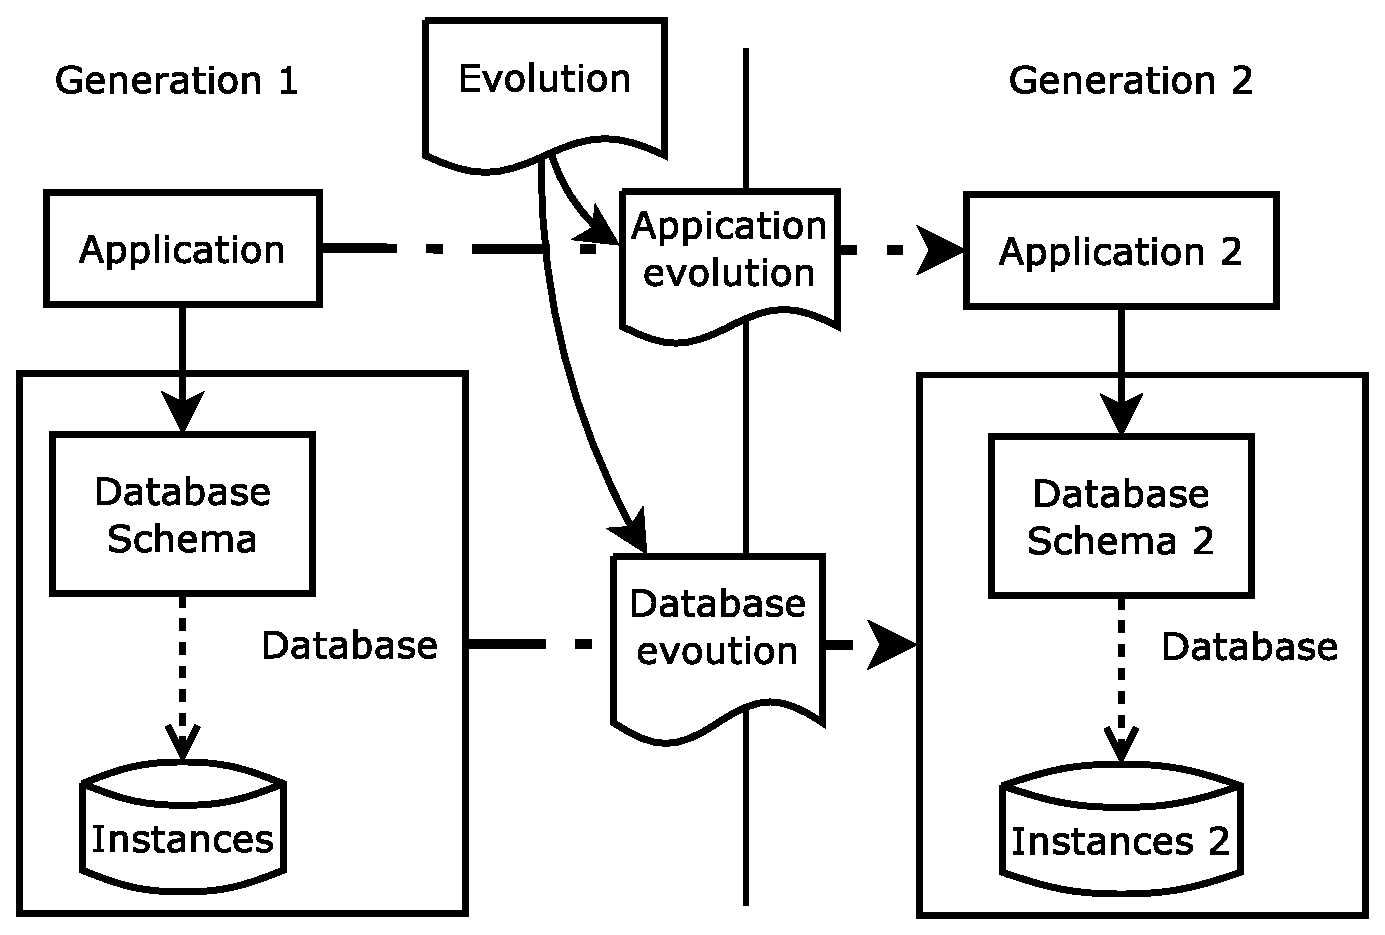
\includegraphics[scale=0.4]{./images/evolution_simple}
	\caption{The evolution of data changes the system on all levels. The figure shows all the components of the evolution process.}
	\label{fig:evolution}
\end{figure}
The evolution of a software is a transformation from one consistent state to another one. These states are called generations of the software and the function which changed the state of a software are called transformations. The evolution consists of change in application and in database as shown in the Figure \ref{fig:evolution}. We focus on situations when the evolution is initiated on the application level (as code refactoring), thus the transformation are designed to conform to the refactoring cases. However a case when the evolution begins on database level is also possible (eg. as a result of database optimization) it is not considered in this paper. 

The evolution of the whole software has to be processed on the both software components - application and database. It means there is a set of application transformations called $AppT$ and a set of database transformations called $DbT$. Because there are needed different parameters for application and database evolution the evolution of database can not be derived from application evolution only. Thus the set of transformation called $E$ is defined to evolve the whole software together with mappings $\Psi$ between $E$ and $AppT$ and $\Phi$ between $E$ and $DbT$ is defined:
\begin{align*}
&	\Psi : E \rightarrow AppT \\
&	\Phi : E \rightarrow DbT
\end{align*}
The set $E$ containing the evolution transformations of a software mets our first goal - a single source of data evolution for the whole software.

The application of a transformation on a software state (evolution) is marked by the $\oplus$ operator:
\begin{align*}
& \oplus \in State \times E \rightarrow State
\end{align*}
and similarly the $\circ$ and the $\bullet$ operators for evolving application and database:
\begin{align*}
& \circ \in Application \times AppT \rightarrow State \\
& \bullet \in Database \times DbT \rightarrow State
\end{align*}
The definition of the evolving operator is inspired by the monads (as used e.g. in Haskell programming language) so the state of the software can be passed from one evolution step to another, which helps us to concatenate evolution transformations.
\begin{align*}
& state(s) \oplus t = \begin{cases}
 	\inference{state(s) = Consistent \; s}{state(sw(\Psi(s, t), \Phi(s,t))} \\ \\
 	\perp
\end{cases}\\ 
& s \in Software, t \in E
\end{align*}
\begin{align*}
& a \circ e = \begin{cases}
 	\inference{!\;consistent(a)}{\perp} \\ \\
 	\inference{consistent(a)}{e(a)} 
\end{cases}\\ 
& a \in Application, e \in AppT
\end{align*}
\begin{align*}
&  d \bullet e = \begin{cases}
 	\inference{!\;consistent(d)}{\perp} \\ \\
 	\inference{consistent(d)}{e(d)} 
\end{cases}\\ 
& d \in Database, e \in DbT
\end{align*}

\section{Software Model}
The model of an ORM software consists of three parts - an application model, a database model and an ORM. The model of application and database creates a type system for both ORM and evolutionary transformations.

The definitions of all parts assume a set $Label$ exists which contains all possible identifiers and each modeled entity is unambiguously identified in the model. Next there is a set $Values$ containing all possible values, which can be used in the model. 

A lot of introduced transformations can be applied on an ordered sets. The application proceeds on set consists in sequential application on set elements:
\begin{align*}
& 	f(x, y) = \begin{cases}
 		\inference{x = \varnothing}{y}\\
 		\inference{|x| > 1}{f(head(x), y) \cup f(tail(x), y}\\\\
 		\inference{|x| = 1}{effect}\\\\
 		\inference{otherwise}{\perp}
 \end{cases}\\\\
& y \in Software \vee y \in Application \vee y \in Database \\
& x \in {y | y \in Type}
\end{align*}
where $x$ is a set of parameters. The effect of a transformation is provided only in next sections as the repetition of sequential application will be redundant. The $otherwise$ branch is consider implicit for all introduced transformations and thus it is not part of transformation definitions too. 


\subsection{Application Model}
\label{sec:appModel}
The application model represents an application persistent layer created using object oriented language and functions which can alter the model. 
\subsubsection{Application Structure}
Each instance in an application is defined according to some class - the class defines the structure of its instances and relationships between them an the rest of the application. The instances are stored in the relational database in our case, therefore we define only the structure of classes in our model. 
\paragraph{Class} Class represents a basic structural unit in the application model. It has a unique name, one or more properties and it can be associated to other classes in the application. 
\begin{align*}
& 	\mathbf{Class} = <label, Property*, Association*> \\
& 	\mathbf{cl} : Label \times Property* \times Association* \rightarrow Class \\\\
& 	\mathbf{name} : Class \rightarrow Label \\
& 	name(cl(l, props, assocs)) = l \\ \\
& 	\mathbf{properties} : Class \rightarrow Property* \\
& 	properties(cl(l, props, assocs)) = props \\ \\
& 	\mathbf{associations} : Class \rightarrow Association* \\ 
& 	associations(cl(l, props, assocs)) = assocs \\ 
& 	l \in Label, props = \{ x | x \in Property\}, assocs = \{ x | x \in Association \}
\end{align*}
Three more function are defined to obtain information about a class - function $primitives$ returns all properties of the class which represent a single value, whereas function $collections$ returns all properties representing collection of values. The last function called $associated$ determine if a class is associated by any other class in an application.
\begin{align*}
&	\mathbf{primitives} : Class \rightarrow Property* \\
&	primitives(cl(l, props, assocs)) = props', \\ 
& props' \subset props,  \forall p \in props' \in cardinality(p) \leq 1 \\ \\
&	\mathbf{collections} : Class \rightarrow Property* \\	
& collections(cl(l, props, assocs)) = props',  \\
& props' \subset props, \forall p \in props' \in cardinality(p) > 1 \\ \\
&	l \in Label, props = \{ x | x \in Porperty\}, assocs  = \{ x | x \in Association\}, \\
& a \in Application
\end{align*}
	 
\paragraph{Property} Property represents a feature of a class which is represented as a primitive type. The property can be mandatory, can have a default value and according to its cardinality it can represent a single value or a collection of values. 
\begin{align*}
&	\mathbf{Property} = <label, AppType, DefaultValue, Cardinality, Mandatory> \\
&	\mathbf{prop} : Label \times AppType \times String \times \mathbb{N^{*}} \times Boolean \rightarrow Property \\ \\
&	\mathbf{name} : Property \rightarrow Label \\
&	name(prop(l, t, val, n, m)) = l \\ \\
&	\mathbf{type} : Property \times AppType \\
&	type(prop(l, t, val, n, m)) = t \\ \\
&	\mathbf{cardinality} : Property \rightarrow \mathbb{N^{*}} \\
&	cardinality(prop(l, t, val, n, m)) = n \\ \\
&	\mathbf{mandatory} : Property \rightarrow Boolean \\
&	mandatory(prop(l, t, val, n, m)) = m  \\ \\
&	l \in Label, t \in AppType, val \in Values, n \in \mathbb{N^{*}}, m \in Boolean 
\end{align*}

\paragraph {Association} Associtation represents a connection between two classes. It has a unique name and the reference is represented by the label of referenced class. The class which owns the association is consider to be the starting class of an association, referenced class is consider to be the ending class of an association. The cardinalities defines the multiplicity of both association ends.
\begin{align*}
&	\mathbf{Association} = <label, classRef, startCardinality, endCardinality> \\
&	\mathbf{assoc} : Label \times Label \times \mathbb{N} \times \mathbb{N} \rightarrow Association\\ \\
&	\mathbf{name} : Association \rightarrow Label \\
&	name(assoc(l, ref, n_1, n_2)) = l\\ \\
&	\mathbf{reference} : Association \rightarrow Label \\
&	reference(assoc(l, ref, n_1, n_2)) = ref\\ \\
&	\mathbf{startCardinality} : Association \rightarrow \mathbb{N} \\
&	startCardinality(assoc(l, ref, n_1, n_2)) = n_1\\ \\
&	\mathbf{endCardinality} : Association \rightarrow \mathbb{N} \\
&	endCardinality(assoc(l, ref, n_1, n_2)) = n_2 \\ \\
&	l, ref \in Label,  n_1, n_2 \in \mathbb{N}, as \in Association
\end{align*}


%TODO: variable types

\paragraph{Application type} Application type ($AppType$) represents primitive type in the application. There are usually defined types such as String, Integer, Boolean etc. in contrast there is only one type in our model, because we focus on structural and data changes and type casting operations are not important for us. The only $AppType$ type is called $APPSTRING$.
\begin{align*}
& \mathbf{AppType} = APPSTRING
\end{align*}

\paragraph{Application} Application is defined as a sequence of classes and it creates the context for all structures used in the software persistent layer.
\begin{align*}
& \mathbf{Application} = (Class*) \\ 
& \mathbf{app} : Class* \rightarrow  Application \\ \\
& \mathbf{classes} \in Application \rightarrow Class* \\
&   classes(app(cs)) = cs  \\\\
& \mathbf{class} : Label \times Application \rightarrow Class   \\ 
&  class(l, a) = c, c \in classes(a) \wedge name(c) = l \\ \\
&  l \in Label,a \in Application, cs = \{x | x \in Class\} 
\end{align*}
The application creates the context for classes so it is possible to determine if a class is associated by other classes or not:
\begin{align*}
& \mathbf{associated} : Label \times Application \rightarrow Boolean \\
& 	associated(l,a) = \begin{cases}
  		\inference{\exists c \in classes(a) \wedge \exists e \in associations(c) : \\ reference(e) = l
  	}{ true } \\\\
 		false
 	\end{cases} \\ \\
&	l \in Label, a \in Application
\end{align*}
The $owningClass$ function returns the class in the model which owns the property or association and it is used during the evolutionary transformation.
\begin{align*}
&	\mathbf{owningClass} : Property \times Application \rightarrow Class  \\ 	
&	owningClass(p, a) = \inference{\exists c \in classes(a) \wedge p \in properties(c)}{c}  \\ \\
&	p \in Property, a \in Application
\end{align*}
\begin{align*}
&	\mathbf{owningClass} : Association \times Application \rightarrow Class  \\
&	owningClass(as, a) = \inference{\exists c \in classes(a) \wedge as \in associations(c)}{c}  \\ \\	
&	as \in Association, a \in Application
\end{align*}


\subsubsection{Application consistency}
The application consistency is based on the structural consistency of its model. Violation of structural consistency are name collisions and non-existing references in associations. The state of an application is:
\begin{align*}
&	\mathbf{consistent} : Application \rightarrow Boolean \\
&	consistent(a) = \begin{cases}
	\inference{\forall c_1, c_2 \in classes(a) : name(c_1) \neq name(c_2) \\ \wedge \forall p_1, p_2 \in properties(c_1) : name(p_1) \neq name(p_2) \\ \wedge \forall a_1, a_2 \in associations(c_1) : name(a_1) \neq name (a_2) \\ \wedge \forall a \in associations(c_1) : \exists c \in classes(a) \wedge name(c) = reference(a)\\
	\wedge \forall p \in properties(c_1), a \in associations(c_1) : name(p) \neq name(a) }{true}\\\\
 	flase
 	\end{cases}\\
&	a \in Application
\end{align*}


\subsection{Database Model}
\label{sec:dbModel}
The relational database consists of database schema which defines the structure of the database and data, which in our ORM system represents stored instances. The database is defined as a tuple:
\begin{align*}
&	\mathbf{Database} = ( Table*, Row* ) \\
&	\mathbf{db} : Tables \times Rows \rightarrow Database \\ \\
&	\mathbf{tables} : Database \rightarrow Tables \\
&	tables(db(tabs, rs)) = tabs \\ \\
&	\mathbf{rows} : Database \rightarrow Rows \\
&	rows(db(tabs, rs)) = rs \\ \\
&	tabs  = \{ x | x \in Table\}, rs  = \{ x | x \in Row\}, l \in Label,d \in Database
\end{align*}
\paragraph{Table} Table represents a basic concept of database schema. It has a unique name, one or more columns and it can be related to other tables in the schema by foreign keys. Rows in the table represents stored data.
\begin{align*}
&	\mathbf{Table} = (label, primaryKey, Column*, ForeignKey*)\\
&	\mathbf{tab} 	: Label \times PrimaryKeys \times Columns \times ForeignKeys \rightarrow Table \\ \\
&	\mathbf{name} : Table \rightarrow Label  \\
&	name(tab(l, pk, cols, fks)) = l \\ \\
&	\mathbf{primaryKey} : Table \rightarrow PrimaryKeys  \\
&	primaryKey(tab(l, pk, cols, fks)) = pk \\ \\
&	\mathbf{columns} : Table \rightarrow Columns  \\
&	columns(tab(l, pk, cols, fks)) = cols \\ \\
&	\mathbf{foreignKeys} : Table \rightarrow ForeignKeys  \\
&	foreignKeys(tab(l, pk, cols, fks)) = fks \\ \\
& l \in Label, pk \in PrimaryKey, cols  = \{ x | x \in Column\}, \\
& fks  = \{ x | x \in ForeignKey\}
\end{align*}

\paragraph{Column} Column defines data values and types which can be part of a table record.
\begin{align*}
&	\mathbf{Column} = (label, DbType, DefaultValue, Constraint*) \\
&	\mathbf{col} : Label \times DbType \times String \times Constraints \rightarrow Column \\ \\
&	\mathbf{name} : Column \rightarrow Label  \\
&	name(col(l, t, val, cons)) = l  \\ \\
&	\mathbf{type} : Column \rightarrow DbType  \\
&	type(col(l, t, val, cons)) = t  \\ \\
&	\mathbf{constraints} : Column \rightarrow Constraints  \\
&	constraints(col(l, t, val, cons)) = cons  \\ \\
&	\mathbf{owningTable} : Column \times Database \rightarrow Table  \\
&	owningTable(c, d) = \inference{\exists tab \in tables(d) \wedge c \in columns(tab)}{tab} \\ \\
& l \in Label, t \in DbType, val \in Values,\\ 
& cons  = \{ x | x \in Constraint\}, c \in Column,d \in Database
\end{align*}

\paragraph{Foreign key} Foreign key is a reference to another table's primary key, it has an unique name and it can be constrained. The value of a foreign key is $\varnothing$ or a non-zero natural number.
\begin{align*}
&	\mathbf{ForeignKey} = < Label, Label, Constraint*> \\ 
&	\mathbf{fk} : Label \times Label \times Constraints \rightarrow ForeignKey \\ \\
&	\mathbf{name} : ForeignKey \rightarrow Label \\
&	name(fk(l, tRef, cons)) = lab  \\ \\
&	\mathbf{reference} : ForeignKey \rightarrow Label  \\
&	reference(fk(l, tRef, cons)) = tRef  \\ \\
&	\mathbf{constaints} : ForeignKey \rightarrow Constraint*  \\
&	constaints(fk(l, tRef, cons)) = cons  \\ \\
&	\mathbf{owningTable} : ForeignKey \times Database \rightarrow Table  \\
&	owningTable(fk, d) = \inference{\exists tab \in tables(d) \wedge fk \in foreignKeys(tab)}{tab}\\\\
&	l, tRef \in Label, cons  = \{ x | x \in Constraint\}, \\ 
& d \in Database, fk = \{ x | x \in ForeignKey\}
\end{align*}


\paragraph{Primary key} Primary key is unambiguous identifier of a record in a table. The primary key is always provided (automatically generated) by the database as a non-zero natural number. Primary key is always defined with constraints $NOTNULL$ and $UNIQUE$. 
\begin{align*}
&	\mathbf{PrimaryKey} =  ( Label, Sequence ) 	\\
&	\mathbf{pk} : Label \times Sequence \rightarrow PrimaryKey \\\\
&	\mathbf{name} : PrimaryKey \rightarrow Label \\
&	name(pk(l, s)) = Id \\\\
&	\mathbf{seq} : PrimaryKey \rightarrow Sequence \\
&   seq(pk(l,s)) = s \\\\
& l \in Label, s \in Sequence
\end{align*}
The sequence generates values of primary key. The new value of a key is obtained by calling the function $next(s)$. The sequence which provides numbers incremented by one is called $s_1$ if the increment is 1, $s_{10}$ if the increment is 10 etc.

\paragraph{Data Types} Database data types $DbType$ represents primitive types in the database. There are usually defined types such as Varchar, Integer, Boolean etc. There is only one type of column values defined in the model called $DBSTRING$. Next the $DBINT$ type is defined for the values of keys.
\begin{align*}
&	\mathbf{DbType} = DBSTRING \; | \; DBINT
\end{align*}

\paragraph{Constraints} There are two types of constraints defined in the model. Both constraints are column constraints - first constraint defines non-empty columns, second constraint defines there has to be unique records in a column or foreign key.
\begin{align*}
&	\mathbf{Constraint} = NOTNULL \; | \; UNIQUE 
\end{align*}

%%%%%%%%%%%%%%%%%%%%%%%%%%%%%%

\subsubsection{Stored Data} 
A database consists not only from schema but also from data which are represented as rows in a table. A table row in our model is a tuple consisting of value pairs, which represents concrete value of concrete column or key. Each row contains a name of a table it belongs to.
\begin{align*}
&	\mathbf{Row} = < Label, N, Pair* > \\
&	\mathbf{row} : Label \times Pairs \rightarrow Row \\ \\
&	\mathbf{refTable} : Row \rightarrow Label \\
&	refTable(row(l, n, ps) = l \\ \\
&	\mathbf{pairs} : Row \rightarrow Pair* \\
&	pairs(row(l, n, ps)) = ps \\ \\
&	\mathbf{idnetifier} : Row \rightarrow N \\
&	idnetifier(row(l, n, ps)) = n \\ \\
&	 l \in Label, ps = \{ x | x \in Pair\}, n \in N
\end{align*}
The value stored in concrete column of the row is represented by a pair, where the $refCol$ is a name of the column, a foreign key or its primary key and $value$ represents concrete value .
\begin{align*}
&	\mathbf{Pair} = < Label, Value > \\
&	[Label \times Value] \rightarrow Pair\\ \\
&	\mathbf{reference} : Pair \rightarrow Label \\
&	reference([l,val]) = l \\ \\
&	\mathbf{value} : Pair \rightarrow Value \\ 
&	value([l,val]) = val \\ \\
&	l \in Label, val \in Value
\end{align*}
The definition of data allows definition of function $contains$ which verify if the table contains data in context of concrete database and $instantiated$, which search for instances of a class with given name and returns true if there are rows for the table in the database.
\begin{align*}
&	\mathbf{contains} : Table \times Database \rightarrow Boolean \\
&	contains(t, d) = \begin{cases}
			\inference{\exists r \in data(d) : refTable(r) = name(t) }{true} \\ \\
		 	false
 		\end{cases} \\ \\
& l \in Label, ps  = \{ x | x \in Pair\}, t \in tables(d), d \in Database
\end{align*}
\begin{align*}
&	\mathbf{instances} : Label \times Row* \rightarrow Row* \\
&	instances(l, r) = \begin{cases}
 		%\inference{r = \varnothing}{\varnothing} \\
 		%\inference{|r| > 1}{instances(head(r)) \cup instances(tail(r))}\\ \\
&		\inference{|r| = 1 \wedge refTable(r) = l}{r}\\\\
& 		\inference{|r| = 1 \wedge refTable(r) \neq l}{\varnothing}
 \end{cases} \\ \\
&	r \in Row*, l \in Label
\end{align*}
\begin{align*}
&	\mathbf{instantiated} : Class \times Software \rightarrow Boolean \\
&	instantiated(c, s) = \begin{cases} \inference{\exists t \in tables(database(s)) : name(t) = name(c) \\ \wedge contains(t, database(s))}{true} \\ \\
  false
 \end{cases} \\ \\
&	 c \in classes(application(s)), s \in Software 
\end{align*}


\subsubsection{Database consistency}
The database consistency is founded on the consistency of structure and consistency between structure and stored values. The conditions for structure consistency are similar as for application structure. The consistency between structure and data is:  each row in a database  refers to a table in database schema and it has to have the structure corresponding to the one defined by a table, moreover the column and foreign key constrains has to be fulfilled  otherwise the database is inconsistent. The consistency of database is:
\begin{align*}
&	\mathbf{consistent} \in Database \rightarrow Boolean \\
&	consistent(d) = \begin{cases}
&		\inference{ \forall t_1, t_2 \in tables(d) : name(t_1) \neq name(t_2) \\ \wedge \forall c_1, c_2 \in columns(t_1) : name(c_1) \neq name(c_2) \\ \wedge \forall f_1, f_2 \in foreignKeys(t_1) : name(f_1) \neq name (f_2) \\ \wedge \forall f \in foreignKeys(t_1) : \exists t \in tables(d) \wedge name(t) = reference(f) \\ \wedge \forall r \in data(d): ( \exists t \in tables(d) : reference(r) = name(t) \\ \wedge \forall p \in pairs(r) :\\ \exists u \in columns(t) \cup foreignKeys(t) \cup primaryKey(t) : \\ reference(p) = name(u) \\ \wedge \forall e \in columns(t) \cup foreignKeys(t) \\ \wedge NOTNULL \in constrain(e) : \exists q \in pairs(r) \\ \wedge name(e) = reference(q)) \\ \wedge \forall g \in columns(t) \cup foreignKeys(t) \\ \wedge UNIQUE \in constrain(g) : \\ \forall u_1, u_2 \in rows(t) : \\ value(pairByName(name(g), u_1) \neq value(pairByName(name(g), u_2) }{true}
 	\\ \\
 	false
 \end{cases}\\
& d \in Database
\end{align*}
 

\subsection{Object-Relational Mapping}
\label{sec:orm}
There are defined functions for object-relational mapping used in this paper. The mapping function itself are not able to create a database from the application as they are mentioned to be used together with evolutionary transformations introduced in section \ref{sec:Evolutionaty-Transformations}.

\paragraph{Mapping of Application} The goal of ORM is usually to determine how an instance is stored in the database. The ORM maps the structure of application classes to database schema. The assumption is a software is evolved continuously and evolutionary transformations produces consistent software, nevertheless to verify consistency of a software we need mapping between an existing application structure and database schema. 
\begin{align*}
&	\mathbf{\rho_{app}} \in Application \rightarrow Database\\
&	\rho_{app}(a) = \inference{state(a) = Consistent \; a}{\begin{gathered}
   db(\varnothing) \bullet addTable(classes(a)) \\ 
	\bullet (\forall c \in classes(a), p \in properties(c) : \\ addProperty(name(c), p) \\
	\bullet (\forall c \in classes(a), e \in associations(c) : \\ addAssociaiton(name(c), e) 
\end{gathered}}\\
& a \in Application
\end{align*}


\paragraph{Mapping of Types} The mapping of types assumes a bijection between application types and database types, otherwise there has to be additional information for type mapping. We focus on structural and data change therefore there is only one type of values in both our models. The mapping is then straightforward:
\begin{align*}
&	\mathbf{\rho_{t}} : AppType \rightarrow DbType  \\
& 	\rho_{t}(APPSTRING) = DBSTRING 
\end{align*}

\paragraph{Mapping of Classes} The class is mapped into a table with  automatically created primary key. The primary key is always created with name Id and of the $\mathbb{N^{*}}$ type. The properties and associations has to be mapped separately.
\begin{align*}
&	\mathbf{\rho_{c}} : Class*  \rightarrow Table* \\
&	\rho_{c}(c) = %\begin{cases}
		%\inference{c = \varnothing}{\varnothing}\\\\
		%\inference{|c| > 1}{\rho_c(head(c)) \cup \rho_c(tail(c))} \\ \\
		\inference{|c| = 1}{table(name(c), primaryKey("Id"), \varnothing, \varnothing)} % \end{cases} 
\\ 	
& c \in Class*
\end{align*}

\subsubsection{Mapping of Properties}
There are two kinds of properties - primitive property with cardinality equal to one is mapped to a column; second kind - collection with cardinality greater than one is mapped to table, thus there are two mapping cases. When the property is mandatory the $NOTNULL$ constraint is added to the column with property value. 

There can occur name collision during mapping in case there are more classes with property representing collection. To avoid that the mapping changes the name of the table representing a collection.
\begin{align*}
&	\mathbf{\rho_p} : Property* \rightarrow Column* \\ \\
&	\rho_{sp}(p) = \begin{cases}
		%\inference{p = \varnothing}{\varnothing}\\
		%\inference{|p| > 1}{\rho_{sp}(head(p)) \cup \rho_{sp}(tail(p))}\\\\
 		\inference{|p| = 1 \wedge cardinality(p) = 1 \wedge !\;mandatory(p)
 			\\ \wedge \exists t : t = table(name(owningClass(p)), d) 
		 }{\begin{gathered}
	  		column(name(p), \rho_t(type(p)), \varnothing )
		\end{gathered}} \\ \\
  		\inference{|p| = 1 \wedge cardinality(p) = 1 \wedge mandatory(p)
			 \\ \wedge \exists t : t = table(name(owningClass(p)), d)
			\\ \wedge \not instanciated(owningClass(p))
		}{\begin{gathered}
 	 		column(name(p), \rho_t(type(p)), NOTNULL ) \\ 
		\end{gathered}}
	\end{cases}\\
&	p \in Property
\end{align*}
\begin{align*}
&	\mathbf{\rho_p} : Property* \rightarrow Table* \\ \\
&	\rho_{cp}(p) = \begin{cases}
		%\inference{p = \varnothing}{\varnothing}\\
		%\inference{|p| > 1}{\rho_{cp}(head(p)) \cup \rho_{cp}(tail(p))}\\\\
     	\inference{|p| = 1 \wedge cardinality(p) > 1 \wedge !\;mandatory(p) \\ 
     		\wedge 	\exists t : t = table(name(owningClass(p)), d)
     		}{\begin{gathered}
     			table(name(t)+name(p), primaryKey("Id"), \\ column("value", \rho_t(type(p)), \varnothing), \\ foreignKey(name(p), 			name(owningClass(p)), NOTNULL) \\
    	\end{gathered}}\\ \\
     	\inference{|p| = 1 \wedge  cardinality(p) > 1 \wedge mandatory(p) \\ 
     		\wedge \exists t : t = table(name(owningClass(p)), d) 
     		}{\begin{gathered}  
     			table(name(t)+name(p), primaryKey("Id"), \\ 
     			column("value", \rho_t(type(p)), NOTNULL), \\ 			foreignKey(name(p), name(owningClass(p)), NOTNULL)
    	 \end{gathered}}
 	\end{cases}\\
& 	p \in Property
\end{align*}

\paragraph{Mapping of Associations} An association is mapped into database as a foreign key in table representing associated class or as a table in case the association cardinality is one to many or many to many. Thus there are two mapping cases as for properties and the same solution is used to avoid name collisions.
\begin{align*}
&	\mathbf{\rho_a} : Association* \rightarrow ForeignKey* \\
&	\rho_a(a) = \begin{cases}
		%\inference{a = \varnothing}{\varnothing}\\
		%\inference{|a| > 1}{\rho_{a}(head(a)) \cup \rho_{a}(tail(a))}\\\\
		\inference{|a| = 1 \wedge  startCardinality(a) = 0 \\ \wedge \exists t : t = table(name(owningClass(p)), d) \\ \wedge \exists u : u = table(reference(a)), d)
		}{
			foreignKey(name(a), name(t),  \varnothing) 
	 	}
  \\ \\
 	 \inference{|a| = 1 \wedge  startCardinality(a) = 1 \\ \wedge \exists t : t = table(name(owningClass(p)), d) \\ \wedge \exists u : u = table(reference(a)), d)
 	 }{ 
		foreignKey(name(a), name(t),  NOTNULL)
	}	 \end{cases}
\\
&	 a \in Association
\end{align*}
\begin{align*} 
&	\mathbf{\rho_a} : Association* \rightarrow Table* \\
&	\rho_a(a) =
% 	  \begin{cases}
 		%\inference{a = \varnothing}{\varnothing}\\
		%\inference{|a| > 1}{\rho_{a}(head(a)) \cup \rho_{a}(tail(a))}\\\\
		\inference{|a| = 1 \wedge   startCardinality > 1 \\ \wedge \exists t \in tables(d) : name(owningClass(p)) = name(t) \\ \wedge \exists e \in tables(d) : name(reference(a)) = name(e)
  		}{\begin{gathered}  
		 table(name(t)+name(a), pk("Id"), \varnothing, \\ foreignKey(owningClass(a),owningClass(a), NOTNULL) \\ foreignkey(reference(a), reference(a), NOTNULL)) 
  		\end{gathered}}  
 	%\end{cases}
\\
&	 a \in Association
\end{align*}

\section{Transformation for Models Manipulation}
The evolution affects both parts of software and as shown in section \ref{sec:evoIntro}. Evolution of software is mapped to transformation specific for application (set $AppT$ of transformations) and database (set $DbT$), both sets are defined in this section.

\subsection{Application Transformation}
This section provide transformations for manipulating the application layer of a software - the $AppT$ set. The set defines common operation for creation, alternation and decomposition of a model (or code).

%\paragraph{Get Property or Association} Functions $findProperty$ and $findAssociation$ returns a property (association) if it exists in given context - application and class of provided name.
%\begin{align*}
%	\mathbf{findProperty} : Label \times Label \times Application \rightarrow Property \\
%	findProperty(l_c, l_p, a) = \inference{\exists c \in classes(a): name(c) = l_c \\ \wedge \exists p \in properties(c) : name(p) = l_p}{p} \\
%	l_c, l_p \in Label, a \in Application
%\end{align*}
%\begin{align*}
%	\mathbf{findAssociation} : Label \times Label \times Application \rightarrow Association \\
%	findAssociation(l_c, l_a, a) = \inference{\exists c \in classes(a): name(c) = l_c \\ \wedge \exists o \in associations(c) : name(o) = l_a}{o} \\
%	l_c, l_a \in Label, a \in Application
%\end{align*}

\paragraph{Add Property} The name collision only has to be verified, before adding a property into an application structure. The transformation inputs are the property to be added and the name of the class the property is going to be added to.
\begin{align*}
& 	\mathbf{addProp} : Label \times Property \times Application \rightarrow Application \\
&	addProp(l, p, a) = \inference{\exists c \in classes(a) : name(c) = l \\ \wedge \forall q \in  properties(c) : name(q) \neq name(p) \\ \wedge \forall e \in associations(c) : name(e) \neq name(p)}{properties(c) \cup p } \\
&	l \in Label, p \in Property, a \in Application
\end{align*}

\paragraph{Add Association} Adding an association into an application structure has to verify if there is no name collision and if there is the associated class present in the application model. 
\begin{align*}
&	\mathbf{addAssoc} : Label \times Association \times Application \rightarrow Application \\
&	addAssoc(l, s, a) = \inference{
	\exists c \in classes(a) : name(c) = l \\
	\wedge \forall f \in associations(c) : name(f) \neq name(s) \\ 	\wedge \forall p \in properties(c) : name(p) \neq name(s) \\ 
	\wedge \exists k \in classes(a) : name(k) = reference(s)}{associations(c) \cup s}\\
&	l \in Labels, s \in Associations, a \in Application
\end{align*}

\paragraph{Add Class} Adding a class is limited to the case when the class has no associations, this is because it simplifies the database migration. The transformation $addClass$ has to verify there is no name collision
\begin{align*}
&	\mathbf{addClass} : Class \times Application \rightarrow Application \\ 
&	addClass(c, a) = \inference{\forall s \in classes(a) : name(s) \neq name(c) \\ \wedge associations(c) = \varnothing }{classes(a) \cup c} \\ \\
&	c \in Class, a \in Application
\end{align*}

\paragraph{Remove Property or Association} The property or association can be simply removed from a class. The transformation inputs (in order) are the name of the property's owning class and the name of property itself.
\begin{align*}
&	\mathbf{remProp} : Label \times Label \times Application \rightarrow Application \\
& 	remProp(l_c, l_p, a) = \inference{\exists c \in classes(a) : name(c) = l_c \\ \wedge \exists p \in properties(c) : name(p) = l_p
	}{properties(c) \setminus p }\\
&	l_c, l_p \in Label, a \in Application 
\end{align*}
\begin{align*}
&	\mathbf{remAssoc} : Label \times Label \times Application \rightarrow Application \\
&	remAssoc(l_c, l_a, a) = \inference{\exists c \in classes(a) : name(c) = l_c \\ \wedge \exists f \in associations(c) : name(f) = l_a }{associations(c) \setminus f} \\
&	l_c, l_a \in Labels, a \in Application
\end{align*}

\paragraph{Remove Class} The class can be removed only in case it is not referenced by any association existing in the application.
\begin{align*}
&	\mathbf{remClass} : Label \times Application \rightarrow Application \\
&	remClass(l, a) = \inference{\exists c \in classes(a) : name(c) = l \\ \wedge !\: associated(c)
	} {classes(a) \setminus c }\\
&	l \in Label,a \in Application
\end{align*}

\paragraph{Rename Property and Association} Both renaming operations can change a name of the property, association respectively if there are no name collisions. The name of owning class, the name of the property (or association) and the new name of the property (association) are inputs of the transformation.
\begin{align*}
&	\mathbf{renProp} : Label \times Label \times Label \times Application \rightarrow Application \\
&	renProp(l_c, l_o, l_n, a) = \inference{\exists c \in classes(a) : name(c) = l_c \\ \wedge \exists p \in properties(c) : name(p) = l_o \\ \wedge \forall e \in properties(c) : name(e) \neq l_n
	}{\begin{gathered}
		p.name = l_n 
	\end{gathered}}\\
&	l_c, l_o, l_n \in Label, a \in Application
\end{align*}
\begin{align*}
&	\mathbf{renAssoc} : Label \times Label \times Label \times Application \rightarrow Application \\
&	renAssoc(l_c, l_o, l_n, a) = \inference{\exists c \in classes(a) : name(c) = l_c \\ \wedge \exists b \in associations(c) : name(b) = l_o \\ \wedge \forall e \in associations(c) : name(e) \neq l_n
	}{\begin{gathered}
		b.name = l_n 
	\end{gathered}}
	\\ & l_c, l_o, l_n \in Label, a \in Application
\end{align*}

\paragraph{Rename Class} When a class is renamed, the name collisions has to be verified and then all referencing associations has to be updated.
\begin{align*}
&	\mathbf{renClass} :  Label \times Label \times Application \rightarrow Application \\
&	renClass(l_o, l_n, a) = \inference{\exists c \in classes(a) : name(c) = l_o \\ \wedge \forall e \in classes(a) : name(e) \neq l_n
	}{\begin{gathered}
		name(c) = l_n \wedge \forall e \in classes(a) \\ \wedge \forall (f \in associations(e) \wedge reference(f) = l_o ) :\\ f.reference = l_n 
	\end{gathered}}\\
& l_o, l_n \in Label, a \in Application	
\end{align*}

\subsection{Database Transformation}
The database is composed from two separated parts - database schema and data. Transformations are defined to manipulate the database schema and to manipulate stored data. Some of presented operations has their origin in SQL queries (especially creation and decomposition), on the other hand some of them cannot be implemented as an SQL query, because of they complexity and conditions verified during theirs execution.

\paragraph{Mapping of Instances} The set $M$ which contains all possible mappings between classes, has to be defined to allow several evolutionary operations. Each mapping represents an ordered set of pairs of instances. These pairs can represent one-to-one (or many) relationship or many-to-many relationship between instances. \begin{align*}
&	m_{l_1, l_2} =  (r_1, r_2)*,\\
& 	r_1 \in instances(l_1, d), r_2 \in instances(l_2, d) \\
&	\forall r_1, r_1 \in instances(l_1, d) \Rightarrow \exists p \in m_{l_1, l_2} \wedge first(p) = r_1 \\
&	\forall r_2, r_2 \in instances(l_2, d) \Rightarrow \exists p \in m_{l_1, l_2} \wedge second(p) = r_2\\\\
&	l_1, l_2 \in Label, r_1, r_2 \in Row, d \in Database
\end{align*}
The mapping $m_{l_1, l_2}$ can be used if there are instances in both tables in database $d$, because there are cases when one of the tables is empty the identity mapping is defined:
\begin{align*}
&	m_{l, l} = (r, r) * \\
& 	\forall r \in instances(l, d) \Rightarrow \exists p \in i_{l} \wedge first(p) = r \\\\
&	l \in Label, r \in Row,  d \in Database
\end{align*}


\paragraph{Comparison of tables} The need to compare two tables during the evolution results into the comparing operator $\cong$. The operator has to be defined for columns and foreign keys too.
\begin{align*}
&	\mathbf{\cong} : Table \times Table \rightarrow Boolean \\
&	t_1 \cong t_2 = \begin{cases}
 		\inference{|columns(t_1)| = |columns(t_2)| \\ \wedge |foreignKeys(t_1)| = |foreignKeys(t_2)| \\ \wedge \forall c \in columns(t_1) \exists e \in columns(t_2) : c = e \\ \wedge \forall f \in foreignKeys(t_1) \exists g \in foreignKeys(t_2) : f = g }{true}\\\\
 false
 \end{cases}\\
& t_1 \in Table, t_2 \in Table
\end{align*}
\begin{align*}
&	\mathbf{\cong} : Column \times Column \rightarrow Boolean \\
&	c_1 \cong c_2 = \begin{cases}
 		\inference{name(c_1) = name(c_2) \\ \wedge type(c_1) = type(c_2) \\ \wedge constraints(c_1) = comstraints(c_2)}{true}
 		\\ \\
		false
 \end{cases}\\
& c_1 \in Column, c_2 \in Column
\end{align*}
\begin{align*}
&	\mathbf{\cong} : ForeignKey \times ForeignKey \rightarrow Boolean \\
&	f_1 \cong f_2 = \begin{cases}
 		\inference{name(f_1) = name(f_2) \\ \wedge reference(f_1) = reference(f_2) \\ \wedge constraints(f_1) = comstraints(f_2)}{true}
 		\\ \\
		false
 \end{cases}\\
& f_1 \in ForeignKey, f_2 \in ForeignKey
\end{align*}

\paragraph{Find pair} The function returns a pair corresponding to given column (or key) name in concrete row.
\begin{align*}
& \mathbf{findPair} : Label \times Row \rightarrow Pair \\
&	findPair(l, r) = \begin{cases}
		\inference{\exists p \in pairs(r) : reference(p) = l}{p} \\ \\
			\varnothing
		\end{cases}\\
&		l \in Label, r \in Row
\end{align*}
\subsubsection{Database Schema Creation}
\paragraph{Add Column} A new column can be add into a table if there are no name collisions. If the column has the $NOTNULL$ constraint, then the default value has to be added to all rows in the table. The inputs of the transformation are name of the table where the column(s) will be added and a sequence of column to add.
\begin{align*}
&	\mathbf{addColumn} : Label \times Column* \times Database \rightarrow Database \\ 	
&	addColum(l, c, d) = \begin{cases}
		%\inference{|c| > 1}{addColumn(l, head(c), d) \bullet addColumn(l, tail(c), d)} \\ \\
		\inference{|c| = 1 \wedge \exists t \in tables(d) \wedge name(t) = l \\ \wedge \forall f \in columns(t) : name(f) \neq name(c) \\ \wedge NOTNULL \not \in constraints(c) }{columns(t) \cup c}\\ \\
		(\inference{|c| = 1 \wedge \exists t \in tables(d) \wedge name(t) = l \\ \wedge \forall f \in columns(t) : name(f) \neq name(c) \\ \wedge NOTNULL \in constraints(c) }{columns(t) \cup c})\\ \bullet addValueToTable(l, [name(c), defVal(c)]) 
%		\\ \\ Inconsistent \;d 
	 \end{cases}\\ 
&	 l \in Label, c \in Column*,d \in Database
\end{align*}

\paragraph{Add Table} The transformation creates a new table in the database. The new table should not contain any foreign keys.
\begin{align*}
&	\mathbf{addTable} : Table* \times Database \rightarrow Database \\ 
&	addTable(t, d) =
		% \begin{cases}
		%\inference{|t| > 1}{d \bullet addTable(head(t)) \bullet addTable(tail(t))}
% \\ \\	
		\inference{|t| = 1 \wedge \forall e \in tables(d) \wedge name(t) \neq name(e) \\ \wedge \forall f \in foreignKeys(t) : \\ \exists e \in tables(d) \wedge name(e) = reference(f) }{tables(d) \cup t}
% \\ \\ 	Inconsistent \;d 
	 %\end{cases}
	 \\ 
&	t = \{x | x \in Table\}, d \in Database
\end{align*}


\subsubsection{Database Schema Alternation}
\paragraph{Alter Column Name} The transformation changes the name of the column identified by its name in given table. The inputs of the transformation are name of the table, name of the column and the new name. 
\begin{align*}
& \mathbf{alterColumn} : Label \times Label \times Label \times Database \rightarrow Database \\
&	alterColumn(l_c, l_o, l_n, d) =
 \inference{\exists t \in tables(a) : name(t) = l_c \\ \wedge \exists c \in columns(t) : name(c) = l_o \\ \wedge \forall e \in columns(t) : name(e) \neq l_n}{\begin{gathered}
c.name = l_n 
\end{gathered}}
 \\
& l_c, l_o, l_n \in Label, d \in Database
\end{align*}

\paragraph{Alter Table} The $alterTable$ function renames a table in  the database.
\begin{align*}
&	\mathbf{alterTable} : Label \times Label \times Database \rightarrow Database \\
&	alterTable(l_o, l_n, d) = \inference{\exists t \in tables(d) : name(d) = l_o \\ \wedge \forall e \in tables(d) : name(e) \neq l_n}{\begin{gathered}
		t.name = l_n \\ \wedge \forall e \in tables(a) \wedge \forall (f \in fks(e) \wedge reference(f) = l_o ) \\ : f.reference = l_n 
	\end{gathered}}\\
&	l_o, l_n \in Label, s \in States, a \in Application, d \in Database
\end{align*}

\paragraph{Copy Column} The transformation creates a copy of a column structure in a another table in the database. The transformation changes only the structure of database - stored data are not changed. The transformation inputs are the name of the table which is the source for the transformation, the name of a column to be copied and the name of the target table. It means the copy operation does not change the name of copied column during its execution. 
\begin{align*}
&	\mathbf{copyColumn} : Label \times Label \times Label \times Database \rightarrow Database \\
&	copyColumn(l_s, l_t, l_c, d) = \begin{cases}
 		\inference{\exists t \in tables(d) : name(t) = l_s \\ \wedge \exists c \in columns(t) : name(c) = l_c \\ \wedge \exists e \in tables(d) : name(e) = l_t  \\ \wedge \forall q \in properties(e) : name(q) \neq l_c}{d \bullet addColumn(l_t, c)} 
	\end{cases} \\
&	l_s,l_t,l_c \in Label \wedge l_s \neq l_t,d \in Database
\end{align*}

\paragraph{Copy Table} The transformation creates a copy of a table in database schema with a given name. The new name has to be different than the old one otherwise the transformation could not be processed.
\begin{align*}
&	\mathbf{copyTable} : Label \times Label \times Database \times Database \\
&	copyTable(l_s, l_t, d) = \inference{\exists t \in tables(d) : name(t) = l_s \\ \wedge \forall e \in tables(d) : name(e) \neq l_t}{\begin{gathered} d \bullet addTable(tab(l_t, primaryKey(t), \\ 
 columns(t), foreignKeys(t)))
\end{gathered}}\\
& l_s, l_t \in Label,  d \in Database
\end{align*}


\subsubsection{Data Manipulation}
\paragraph{Insert row} The function allow to insert a row or rows into the database.
\begin{align*}
&	\mathbf{insertRow} : Row* \times Database \rightarrow Database \\
&	insertRow(r, d) = \begin{cases}
			%\inference{|r|>1}{d \bullet insertRow(head(r), d) \bullet insertRow(tail(r), d)} \\ \\
		 	\inference{|r|=1 \wedge \exists t \in tables(d) : name(t) = reference(r) \\ \wedge \forall e \in instances(t, d) : idnetifier(e) \neq idnetifier(r)}{data(d) \cup r} 
		 	%\\ \\	 Inconsistent \; d
		 \end{cases}	\\
&		 r = \{ x | x \in Row\},d \in Database
\end{align*}

\paragraph{Insert Value} The function inserts a new pair or pairs into an existing row.
\begin{align*}
&	\mathbf{insertValue} : Label \times N \times Pair* \times Database \rightarrow Daatabase \\
&	insertValue(l, n, p, d) = \begin{cases}
 		%\inference{|p| > 1}{\begin{gathered} 	d \bullet insertValue(r, head(p), d) \\ \bullet insertValue(r, tail(p), d)\end{gathered}}   \\ \\
 		\inference{|p| = 1 \wedge 
 		\\ \wedge \exist r \in instances(l, d) : value(findPair("Id", r)) = n
 		\\ \wedge \exists t \in tables(d) : name(t) = l, 
 		\\ \wedge \exists c \in columns(t) : reference(p) = name(c) 
 		\\ \wedge \forall e \in pairs(r) :\\  reference(e) \neq reference(p) }{pairs(r) \cup p} 
 		%\\ \\ Inconsistent \; d
 		\end{cases} \\
& r = \{ x | x \in Row\}, p = \{ x | x \in Pair\},d \in Databases
\end{align*}

\paragraph{Add Value To Table} The function appends a pair to all rows of a table with given name.
\begin{align*}
&	\mathbf{addValueToTable} : Label \times Pair \times Database \rightarrow Database \\
&	addValueToTable(l, p, d) = \begin{cases}
 		\inference{\exists t \in tables(d) : name(t) = l}	{\begin{gathered}
		d \bullet (\forall r \in instances(l, d) \\ : insetValue(reference(r), keyValue(r), p) \\ \bullet addValueToTable(tail(instances(l, d)), p, d))
	\end{gathered}} 
 	\end{cases}\\ 
& 	l \in Label, p \in Pair,  d \in Database
\end{align*}

\paragraph{Copy Value} The function copy value from one column in a table to another column in the same or in another table - according to provided mapping. First argument of the transformation is the name of the source table, the second one is the target table, then there are names of source column and target column, finally the mapping between rows (stored instances) has to be provided.
\begin{align*}
&	\mathbf{copyValue} : Label \times Label \times Label \times Label \times (Row \times Row) \times Database \rightarrow Database \\
&	copyValue(l_s, l_t, l_{sc}, l_{tc} o_{l_s, l_t}, d) = \begin{cases}
		\inference{\exists t_s \in tables(d) : name(t_s) = l_s, \\ t_t \in tables(d) : name(t_t) = l_t, \\ c \in columns(t_s) : name(c) = l_{sc}, \\ e \in columns(t_t) : name(e) = l_{tc}}{\begin{gathered}
		\forall	p \in m_{l_s, l_t} :	d \bullet insertValue(name(second(p)), keyValue(second(p)), \\ [l_{tc},value(findPair(l_{sc}, first(p)))])
		\end{gathered}}
 	\end{cases} \\
& 	l_s, l_t, l_{sc}, l_{tc} \in Label, d \in Database
\end{align*}

\paragraph{Copy rows} The function $copyRow$ creates a copy of a source table content in another table with the same structure. 
\begin{align*}
&	\mathbf{copyRow} : Label \times Label \times (Row \times Row) \times Database \rightarrow Database \\
&	copyRow(l_s, l_t, m_{l_s, l_t}, d) = \begin{cases}
 	%\inference{|m_{l_s, l_t}| = \varnothing}{d} \\\\
 	%\inference{|m_{l_s, l_t}| > 1}{\begin{gathered} d \bullet copyRow(l_s, l_t, head(M_{l_s, l_t})) \\ \bullet copyRow(l_s, l_t, tail(m_{l_s, l_t})) \end{gathered}}
 	\inference{|m_{l_s, l_t}| = 1 \\ \wedge \exists t_s, t_t \in tables(d) : name(t_s) = l_s, name(t_t) = l_t \\ \wedge t_s \cong t_t }{d \bullet insertRow(row(l, pairs(first(m_{l_s, l_t}))), d)} \\\\
  \end{cases} \\
&  l_s, l_t \in Label, d \in Database, m_{l_s, l_t} \in M
\end{align*}

\subsubsection{Database decomposition}
\paragraph{Remove a value}  The approach introduced in this paper has to  preserve data and information, nevertheless there are cases when data can be deleted from the database without data lost as they are e.g. already copied in another column as the understanding of data changed in the whole software, therefore we defined two transformations - one removes a single value from a row, second removes whole row (instance) from the software.
\begin{align*}
&	\mathbf{dropValue} : Label \times Row \times Database \rightarrow Database \\
&	dropValue(l, r, d) = \inference{\exists p \in pairs(r) : reference(p) = l}{pairs(r) \setminus p}\\ 
& l \in Label, r : Row \wedge r \in data(d), d \in Database
\end{align*}
\begin{align*}
&	\mathbf{dropRow} :  Row*  \times Database \rightarrow Database\\
&	dropRow(r, d) = \inference{|r|=1}{data(d) \setminus r}	\\ 
& l \in Label, r \in Row \wedge r \in data(d), d \in Database
\end{align*}


\paragraph{Remove table, column or key} The functions removes a table, column or key if there are no stored data. This is because the data lost is undesirable in case of evolution. The consistency of foreign keys references has to be verified too in case a table is removed.  There are defined two variants of remove transformations for each model entity - one preserves data, the other removes data too.
\begin{align*}
&	\mathbf{dropTable} : Label \times Database \rightarrow Database \\
&	dropTable(l,d) = \inference{ \exists t \in tables(d) : name(t) = l  \\ \wedge \forall r \in data(d) : owningTable(r) \neq l \\  \wedge (\forall j \in tables(d) \wedge f \in foreignKeys(j) : reference(f) \neq l) }{ tables(d) \setminus \rho(c)}\\
& l \in Label, d \in Database
\end{align*}
\begin{align*}
&	\mathbf{dropTableAndData} : Labe \times Database \rightarrow Database \\
&	dropTableAndData(l, d) = \inference{\exists t \in tables(d) \\ \wedge ! \; associated(t, d)}{\begin{gathered}
	(\forall r \in instances(t,d) : dropRow(r, d))\\ \bullet dropTable(t,d)
\end{gathered}}
	\\& l \in Label, d \in Database
\end{align*}

\begin{align*}
&	\mathbf{dropColumn} : Label \times Label \times Database \rightarrow Database \\
& 	dropColumn(l, l_p, d) = \inference{ \exists t \in tables(d) : name(t) = l \\ \wedge \exists c \in columns(t) : name(c) = l_p \\ \wedge \forall e \in  pairs(r), r \in instances(t, d) : \\ reference(e) \neq l_p \vee value(e) = \varnothing  }{columns(t) \setminus c}\\
&	 l , l_p\in Label, d \in Database 
\end{align*}
\begin{align*}
&	\mathbf{DropColumnAndData} : Label \times Label* \times Database \rightarrow Database \\
&	DropColumnAndData(l_c, ps, d) = \\
&= \begin{cases}
 	%\inference{ps = \varnothing}{d}\\
 	 %\inference{|ps| >1}{\begin{gathered} 	d \bullet DropColumnAndData(l_c, head(ps), d) \\ \bullet DropColumnAndData(l_c, tail(ps), d) \end{gathered}} \\ \\
 	(\inference{|ps| = 1 \\ \wedge \exists t \in tables(d) \\ \wedge \exists c \in columns(t) : name(c) = l_c}{\begin{gathered}
	 	(\forall r, r \in instances(d) \wedge reference(r) = l_c: \\d \bullet dropValue(ps, r)) \end{gathered}}) \\ \bullet dropColumn(l_c)  
 \end{cases}
	\\
&	l_c \in Label, ps = \{ x | x \in Label\}, d \in Database
\end{align*}

\begin{align*}
&	\mathbf{dropKey} : Label \times Label \times Database \rightarrow Database \\
&	dropKey(l, l_p, d) = \inference{ \exists t \in tables(d) : name(t) = l \\ \wedge \exists c \in foreignKeys(t) : name(c) = l_p \\ \wedge \forall e \in  pairs(r), r \in instances(t, d) : \\ reference(e) \neq l_p \vee value(e) = \varnothing  }{foreignKeys(t) \setminus c}\\
&	 l, l_p \in Label, d \in Database 
\end{align*}
\begin{align*}
&	\mathbf{DropKeyAndData} : Label \times Label* \times Database \rightarrow Database \\
&	DropKeyAndData(l_f, ps, d) = \\
& = \begin{cases}
 	%\inference{ps = \varnothing}{d}\\
 	 %\inference{|ps| >1}{\begin{gathered} 	d \bullet DropColumnAndData(l_c, head(ps), d) \\ \bullet DropColumnAndData(l_c, tail(ps), d) \end{gathered}} \\ \\
 	(\inference{|ps| = 1 \\ \wedge \exists t \in tables(d) \\ \wedge \exists f \in foreignKeys(t) : name(f) = l_f}{\begin{gathered}
	 	(\forall r, r \in instances(t,d) \wedge reference(r) = l_f: \\d \bullet dropValue(ps, r)) \end{gathered}}) \\ \bullet dropKey(l_f)  
 \end{cases}
	\\
&	l_f \in Label, ps = \{x | x \in Label \}, d \in Database
\end{align*}



\section{Evolutionaty Transformations}
\label{sec:Evolutionaty-Transformations}
The set of all possible data evolution cases $E$ was defined in Section \ref{sec:evoIntro}. The semantic of transformations in the set $E$ is defined by their interpretation on individual software components. This section provides an overview of basic transformations (evolution cases) and theirs interpretation on the application and the database. The section starts with simple transformations as the complex one can be often implemented as theirs concatenation. The transformations are divided into three groups - first group creates the structure of a software, second group removes parts of a software structure and third group is able to alter the structure.

It is important to notice that each instance of the software has different data in its database. It means that the evolution can be feasible only for some instances of the software and thus proposed transformation has to be always interpreted in context of the whole software.


\subsection{Software Creation}
There are defined three transformations which are able to create a software: $addProperty$, $addAssociation$,  $newClass$. These three transformations can be used to create a software from a scratch. The last of them has no impact on stored data, whereas the rest of them can in some cases.
\paragraph{Add Property} Adding a property to database can change not only structure but stored data too, because a mandatory property can be added into a class with already existing instances, then a default value has to be added to all existing instances.
\begin{align*}
&	\mathbf{addProperty} : Label \times Property \times State \rightarrow State \\
&	\Psi(s, addProperty(l, p)) = application(s) \circ addProp(l,p) \\
&	\Phi(s, addProperty(l, p)) = \\
& = \begin{cases}
    		\inference{cardinality(p) \leq 1}{database(s) \bullet addColumn(l, \rho(p,d), d)} \\ \\
	    \inference{ \exists t \in tables(d) : name(t) = name(owningClass(p)) \\ \wedge mandatory(p) \wedge instantiated(owningClass(p)) \\ \wedge cardinality(p) \leq 1}{\begin{gathered}
   database(s) \bullet addTable(\rho(p,d), d) \\ \bullet \forall r \in row(owningClass(p)) :\\ insertRow(row(name(p), ["value", defaultValue(p)], \\ [name(p), value(primaryKey(r))])) 
    \end{gathered} } 
   \end{cases}\\
&	s \in State, l \in Label, p \in Properties
\end{align*}


\paragraph{Add association} Adding an association into a database is complicated because of already existing instances. When an association between classes is added the instances of both classes has to be connected on the database level via foreign key or connection table. The information about pairing has to be provided by the user in form of set of instances pairs, because the model does not contain enough information. 
\begin{align*}
& \mathbf{addAsociation} : Label \times Association \times (Row \times Row) \times State \rightarrow State \\
& \Psi(s, addAsociation(l, a, m_{l_1, l_2})) = application(s) \circ addAssoc(l, a) \\
& \Phi(s, addAsociation(l, a, m_{l_1, l_2})) = \\
& =\begin{cases}
	\inference{ \exists t_s, t_t \in tables(d) : name(t_s) = l\\ 		\wedge name(t_t) = reference(a) \\ \wedge \forall f \in foreignKeys(t_t) \cup columns(t_t) \\: name(f) \neq name(a) \\ startCardinality(a) \leq 1}{\begin{gathered}
		database(s) \\ \bullet addForeignKey(name(t_t), \rho(a,d), d) \\ \bullet \forall r \in m_{l_1, l_2} : \\
		insertValue(name(t_t), value(primaryKey(second(r))), [name(a), value(primaryKey(first(r)))])
	\end{gathered}}
 \\ \\
	\inference{ \exists t_s, t_t \in tables(d) : name(t_s) = l \\ \wedge name(t_t) = reference(a) \\ \wedge startCardinality(a) > 1}{\begin{gathered} 
	database(s) \bullet addTable(\rho(a,d),d) \\ \bullet \forall r \in m_{l, reference(a)} :
	\\ insertRow(\\ row(name(owningClass(a)) + name(a), \\ [name(t_s), value(primaryKey(first(r)))]\\ [name(t_t), value(primaryKey(second(r)))]))
	\end{gathered}} 
\end{cases}\\
& s \in Software, l_1, l_2 \in Label, m_{l, reference(a)} \wedge l_2 = reference(a)
\end{align*}

\paragraph{Add Class} The $insertClass$ operation changes the structure of the database schema only, because the $insertAssoc$ transformation needs a mapping function to work properly, which is not part of the $newClass$ definition. The situation reflect the modeling praxis when the structure of a class is defined and then its associations are created.
\begin{align*}
& \mathbf{newClass} : Class \times State \rightarrow State \\
& \Psi(s, newClass(c)) = application(s) \circ addClass(c) \\
& \Phi(s, newClass(c)) = database(s)  \bullet addTable(\rho(c,d)) \\ 
& \bullet addColumn(name(c), \{\forall r \in singleProperties(c) | \rho(r,d)\}, database(s)) \\
& \bullet addTable(name(c), \{\forall r \in collections(c) | \rho(r,database(s))\})  \\
& s \in Software, c \in Class
\end{align*}




\subsection{Software Decomposition}
The removal of class, property or association is limited only by the constraints given in application or database transformations. The main constraint is there has to be no data, which can be lost during removal. 
\paragraph{Remove class}
\begin{align*}
&	\mathbf{RemoveClass}: Label \times Software \rightarrow State  \\
&	\Psi RemoveClass(l, s) = applications(s) \circ remClass(l) \\
&	\Phi RemoveClass(l, s) = database(s) \bullet dropTable(l) \\
&	l \in Label, s \in Software 
\end{align*}

\paragraph{Remove property}
\begin{align*}
&	\mathbf{RemoveProperty} : Label \times Label \times State \rightarrow State \\
&	\Psi RemoveProperty(l, l_p, s) =  applications(s) \circ  remProp(l, l_p) \\
&	\Phi RemoveProperty(l, l_p, s) = \\
& \begin{cases}
		 \inference{\exists c \in classes(application(s)) : name(c) = l\\ 
		\wedge \exists p \in properties(c) : name(p) = l \\ \wedge cardinality(p) \leq 1}{database(s) \bullet dropColumn(l, l_p)}  \\\\
		 \inference{\exists c \in classes(application(s)) : name(c) = l\\ 
		\wedge \exists p \in properties(c)  : name(p) = l \\ \wedge cardinality(p)>1}{database(s) \bullet dropTable(name(owningClass(p)+l)}
 	\end{cases}\\
&	l, l_p \in Label, s \in State
\end{align*}

\paragraph{Remove Property and its Data} The $RemovePropertyAndData$ transformation helps to remove a property together with data stored in the database. The evolution can cause data and information lost, to prevent this the transformation $RemovePropertyAndData$ should be used carefully.
\begin{align*}
&	\mathbf{RemovePropertyAndData} : Label \times Label* \times State \rightarrow State \\
&	\Phi(RemovePropertyAndData(L_c, ps), s) = application(s)\\ 
&  \circ remProperty(l_s, ps) \\
&	\Psi(RemovePropertyAndData(L_c, ps), s) = \\
& = \begin{cases}
		%\inference{ps = \varnothing}{d}\\
		%\inference{|ps| > 1}{\begin{gathered} database(s) \\ \bullet RemovePropertyAndData(L_c, head(ps)) \\ \bullet RemovePropertyAndData(L_c, tail(ps)) 	\end{gathered}}\\\\
 		\inference{\exists c \in classes(application(s)) : name(c) = l\\ 	\wedge \exists p \in properties(c) : name(p) = l \\ \wedge cardinality(p) \leq 1}{database(s) \bullet DropColumnAndData(l_c, ps)}\\\\
 	\inference{\exists c \in classes(application(s)) : name(c) = l\\ 	\wedge \exists p \in properties(c) : name(p) = l \\ \wedge cardinality(p) > 1}{database(s) \bullet RemoveTableAndData(name(owningClass(p))+l_c, ps)}
 \end{cases}
	\\
&	l_c \in Label, ps = \{x | x \in Label\}, s \in State
\end{align*}

\paragraph{Remove association} 
\begin{align*}
&    \mathbf{RemoveAssociation} : Label \times Labels \times State \rightarrow State \\ 
&    \Psi RemoveAssociation(l, l_a, s) = application(s) \circ remAss(l, l_a) \\
&    \Phi RemoveAssociation(l, l_a, s) = \\
&= s\begin{cases}
     	\inference{\exists c \in classes(application(s)) : name(c) = l \\
     	\wedge \exists a \in associaions(c) : name(a) = l_a  \\
     	\wedge startCardinality(a) \leq 1 \\}{database(s) \bullet dropForeignKey(l_a, reference(a))} \\\\
     	\inference{\exists c \in classes(application(s)) : name(c) = l \\
     	\wedge \exists a \in associaions(c) : name(a) = l_a  \\
     	\wedge startCardinality(a) > 1}{database(s) \bullet dropTable(name(owningClass(a))+l_a)} 
     \end{cases}\\
&    l_c, l_a \in Labels, s \in State
\end{align*}

\paragraph{Remove Association and its Data} The $RemoveAssociationAndData$ transformation helps to remove a property together with data stored in the database. The evolution can cause data and information lost, to prevent this the transformation $RemoveAssociationAndData $ should be used carefully.
\begin{align*}
&	\mathbf{RemoveAssociationAndData} : Label \times Label* \times State \rightarrow State \\
&	\Phi(RemoveAssociationAndData(L_c, ps), s) = application(s)\\ 
& \circ remAssociation(l_s, ps) \\
&	\Psi(RemoveAssociationAndData(L_c, ps), s) = \\
&=  \begin{cases}
		%\inference{ps = \varnothing}{d}\\
		%\inference{|ps| > 1}{\begin{gathered}			database(s) \\ \bullet RemoveAssociationAndData(L_c, head(ps)) \\ \bullet RemoveAssociationAndData(L_c, tail(ps)) \end{gathered}}\\\\
 		\inference{\exists c \in classes(application(s)) : name(c) = l\\ 	\wedge \exists a \in associations(c) : name(a) = l \\ \wedge startCardinality(p) \leq 1}{\begin{gathered}
	database(s) \\ \bullet RemoveForeignKeyAndData(reference(a), ps)
\end{gathered}}
 		\\\\
 	\inference{\exists c \in classes(application(s)) : name(c) = l\\ 	\wedge \exists a \in associations(c) : name(a) = l \\ \wedge startCardinality(a) > 1}{\begin{gathered}
	database(s) \\\bullet RemoveTableAndData(l_c + reference(a), ps)
\end{gathered}}
 \end{cases}
	\\
&	l_c \in Label, ps : Label*, s \in State
\end{align*}


\subsection{Software Alternation}
Alternation of a software is limited to renaming functions in our model.
\paragraph{Rename Class}
\begin{align*}
& \mathbf{RenameClass} : Label \times Label \times State \rightarrow State \\ 
& \Psi(RenameClass(l_o, l_n), s) = application(s) \circ renClass(l_o, l_n) \\
& \Phi(RenameClass(l_o, l_n), s) = database(s) \bullet alterTable(l_o, l_n) \\ \\
\end{align*}

\paragraph{Rename Property}
\begin{align*}
&	\mathbf{RenameProperty} : Label \times Label \times Label \times State \rightarrow State \\ \\
& \Psi(RenameProperty(l_c, l_o, l_n, s)) = application(s) \circ renProp(l_c, l_o, l_n) \\
& \Phi(RenameProperty(l_c, l_o, l_n, s)) = \begin{cases}
 	\inference{\exists c \in classes(application(s)) : name(c) = l\\ 
		\wedge \exists p \in properties(c) : name(p) = l_o \\
 	cardinality(p) \leq 1}{database(s) \bullet alterColumn(l_c, l_o, l_n))} \\\\
 	\inference{\exists c \in classes(application(s)) : name(c) = l\\ 
		\wedge \exists p \in properties(c) : name(p) = l_o \\
 	cardinality(p) > 1}{\begin{gathered}
		database(s)\\ \bullet alterTable(name(owningClass(p)+l_o, l_n, database(s))
\end{gathered}}
 \end{cases}\\
& l_c, l_o, l_n \in Label,  s \in State
\end{align*}



\paragraph{Rename Association}
\begin{align*}
& \mathbf{RenameAssociation} : Label \times Label \times Label \times State \rightarrow State \\
& \Psi(RenameAssocaiation(l_c, l_o, l_n), s) = application(s) \circ renAssoc(l_c, l_o, l_n)\\
& \Phi(RenameAssocaiation(l_c, l_o, l_n), s) = \begin{cases}
	\inference{\exists c \in classes(application(s)) : name(c) = l\\ 
		\wedge \exists a \in associations(c) : name(a) = l_o 
	\\ \wedge startCardinality(a) > 1 }{\begin{gathered}
		database(s) \\ \bullet alterTable(name(owningClass(a)) + l_o, l_n)
\end{gathered}}\\ \\
  \inference{\exists c \in classes(application(s)) : name(c) = l\\ 
		\wedge \exists a \in associations(c) : name(a) = l_o 
	\\ \wedge startCardinality(a) \leq 1 }{\begin{gathered}
database(s) \\ \bullet alterForeignKey(endClass(a) ,l_c, l_o, l_n)
\end{gathered}}
 \end{cases} \\
&	l_c, l_o, l_n \in Label, a \in Application, s : Sate
\end{align*}


\paragraph{Copy Property}
All transformations described earlier does change primary the structure of an application. Therefore we define  the transformation for copying a property from one class to another. Copy property is the basic way to move data among instances of different classes. Note the transformation does not move a single value, but it move the values for all instances in the software.

There are two possible implementation of transformation for copying property, first implementation $CopyPropertyStructure$ copies only the structure of a property on the database level, the second implementation $CopyProperty $ copies both structure and data of the property.
\begin{align*}
&	\mathbf{CopyPropertyStructure} : Label \times Label \times Label \times State \rightarrow State \\
&	\Psi(CopyPropertyStructure(l_s, l_t, l_p, s) = \inference{\exists c \in classes(s) : name(c) = l_s \\ \wedge \exists p \in properties(c) : name(p) = l_p }{application(s) \circ addProp(l_t, p)} 
	\\\\
&	\Phi(CopyPropertyStructure(l_s, l_t, l_p, s) = \begin{cases}
    \inference{\exists p \in properties(c), c \in classes(s) : \\ name(p) = l_p \wedge cardinality(p) \leq 1 }{\begin{gathered}
			database(s) \bullet copyColumn(l_s, l_t, l_p) 			\end{gathered}} \\ \\
		\inference{\exists p \in properties(c), c \in classes(s) : \\ name(p) = l_p \wedge cardinality(p) > 1}{\begin{gathered}
			database(s) \bullet copyTable(l_s + l_p, l_t + l_p) 			\end{gathered}}
 \end{cases}\\
& l_s, l_t, l_p \in Label, s \in State
\end{align*}

\begin{align*}
&	\mathbf{CopyProperty} : Label \times Label \times Label \times (Row \times Row) \times State \rightarrow State \\
&	\Psi(CopyProperty(l_s, l_t, l_p, m_{l_s, l_t}), s) = \inference{\exists c \in classes(s) : name(c) = l_s \\ \wedge \exists p \in properties(c) : name(p) = l_p }{application(s) \circ addProp(l_t, p)} 
	\\\\
&	\Phi(CopyProperty(l_s, l_t, l_p, m_{l_s, l_t}), s) = \begin{cases}
		\inference{\exists p \in properties(c), c \in classes(s) : \\ name(p) = l_p \wedge cardinality(p) \leq 1 }{\begin{gathered}
			database(s) \bullet copyColumn(l_s, l_t, l_p) \\ \bullet copyValue(l_s, l_t, l_p, l_p, m_{l_s, l_t}) 
			\end{gathered}} \\ \\
		\inference{\exists p \in properties(c), c \in classes(s) : \\ name(p) = l_p \wedge cardinality(p) > 1}{\begin{gathered}
			database(s) \bullet copyTable(l_s + l_p, l_t + l_p) \\ \bullet copyRow(l_s + l_p, l_t + l_p, m_{l_s, l_t}) 
			\end{gathered}}
 \end{cases}\\
& l_s, l_t, l_p \in Label,  m_{l_s, l_t}) \in M, s \in State
\end{align*}
With the copy property transformation defined we are able to define advanced evolution scenarios.

%\paragraph{Change Cardinality}
%$$\rho_{CcP} : Property \times \mathbb{N^{*}} \times Application \rightarrow Property $$
%$$\rho_{cardA} : Association \times \mathbb{N^{*}} \times Application \rightarrow Association $$

\section{Advanced Refactoring Cases}
The refactoring cases presented in this section were chosen according to the refactoring statistics provided by Eclipse, concretely Move property and Extract/Inline class were chosen to prove the capabilities of defined transformations and next complex refactoring case - merge of two classes - is presented.
\paragraph{Move Property}
The aim of the move property transformation is to change two classes - one will get a new property, the other will lost a property. An example of such transformation is merging information from one class to another. The implementation of move property transformation is based on copy property transformation. Its inputs are the name of source class, the name of target class and the sequence of names of properties to be moved from source to target, finally the mapping between instances of source and target class.
\begin{align*}
&	\mathbf{MoveProperty} : Label \times Label \times Label* \times (Row \times Row) \times State \rightarrow State \\
&	s \oplus MoveProperty(l_s, l_t, ps, m_{l_s, l_t}) =
% \begin{cases}
%	\inference{|ps| = \varnothing}{state(s)}\\\\
%	\inference{|ps| > 1}{\begin{gathered} 	s \oplus MoveProperty(l_s, l_t, head(ps), m_{l_s, l_t}) \\ \oplus MoveProperty(l_s, l_t, tail(ps), m_{l_s, l_t}) \end{gathered}}
 	\inference{|ps| = 1 }{\begin{gathered} s \oplus CopyProperty(l_s, l_t, ps, m_{l_s, l_t}) \\ \oplus RemovePropertyAndData(l_s, ps)
\end{gathered}}
% \end{cases}
	\\
&	l_s, l_t \in Label, ps \in Label*,  m_{l_s, l_t} \in M, s \in State
\end{align*}
Although the $MoveProperty$ transformation contains the transformation $RemovePropertyData$ its execution preserve data and information as the information has been already copied. 

\paragraph{Extract and Inline Class}
The extract and inline class are two opposite transformations. First of them extract a class from existing class, second of them merges two classes into one.
\begin{align*}
&	\mathbf{Extract} : Label \times Label \times Label \times (Row \times Row) \times State \rightarrow State \\
&	s \oplus Extract(l_s, l_n, ps, m_{l_s, l_s}) = \begin{cases}
	\inference{|ps| = 1}{\begin{gathered}
		s \oplus addClass(cl(l_n, \varnothing, \varnothing)) \\ \oplus MoveProperty(l_s, l_n, ps, m_{l_s, l_s}) \end{gathered}}\\\\
	%\inference{|ps| > 1}{\begin{gathered} 	s \oplus Extract(l_s, head(ps), l_n) \\\oplus Extract(l_s, tail(ps), l_n) \end{gathered}}\\\\
	% \inference{|ps| = \varnothing}{state(s)}	 
 \end{cases}
	\\
&	l_s, l_n \in Label, ps ={ x | x  \in Label},  s \in State 
\end{align*}
The opposite transformation $Inline$ gets the name of a class to inline and the name of target class. The result of the transformation is a merge of information from two classes in the target class, the source class is removed. The important condition of feasibility is there is no name collision among properties in both classes.
\begin{align*}
&	\mathbf{Inline} : Label \times Label \times (Row \times Row) \times State \rightarrow State \\
&	s \oplus Inline(l_s, l_t, m_{l_s, l_t}) = \inference{\exists c_s \in classes(application(s)) : name(c_s) = l_s \\
\wedge \exists c_t \in classes(application(s)) : name(c_t) = l_t \\
\wedge \forall p_s \in properties(c_s), p_t \in properties(c_t) : name(ps) \neq name(p_t) \\
\wedge !\:associated(l_s, s)   }{\begin{gathered}
	s \oplus MoveProperty(l_s, l_t, ps, m_{l_s, l_t}) \\ \oplus RemoveClass(l_s) 
\end{gathered}
}\\
& l_s, l_t \in Label, m_{l_s, l_t} \in M, s \in State, \\ 
& ps = \{x | x \in \forall c \in classes(application(s)) : \forall p \in properries(c) : name(p))\}
\end{align*}

\paragraph{Merge of Classes} There occur situations when there is a need to merge two classes and the inlining transformation cannot be used because of name collisions among properties in such a case the $merge$ transformation can be used. It can be used in case structure of both classes (respectively tables) is equals. The transformation creates new rows in the new table - the primary keys from origin instances are replaced by a new ones.
\begin{align*}
&	\mathbf{merge} : Label \times Label \times Label \times State \rightarrow State \\
&	\Phi(s, merge(l_1, l_2, l_n) = \inference{
		\exists c_1, c_2 \in classes(application(s)) \wedge 
		equals(c_1, c_2)}{\begin{gathered}
			application(s) \circ addClass(cl(ln, \varnothing, \varnothing)\\ \circ (\forall p \in properties(c_1) : addProperty(l_n, p)) \\ \circ (\forall a \in associations(c_1): addAssociation(l_n, a))
		\end{gathered}} \\\\
&	\Psi(s, merge(l_1, l_2, l_n) = \inference{\exists t_1, t_2 \in tables(database(s)) : \\ name(t_1) = l_1 \wedge name(t_2) = l_2 \\
\wedge ! \: referenced(t_1, d) \wedge ! \: referenced(t_2, d) }{\begin{gathered}
	 database(s) \bullet addTable(l_n, \mathbf{X}, \varnothing, \varnothing) \\ \bullet (\forall c \in columns(t_1) : addColumn(l_n, c)) \\ \bullet (\forall f \in foreignKeys(t_1) : addForeignKey(l_n, f)) \\ \bullet (\forall r \in instances(t_1, database(s)) \cup instances(t_2, database(s)) :  \\ insertRow(l_n, row(l_n, next(seq(key(l_n))), pairs(r)))) 
\end{gathered}}\\
& l_1, l_2, l_n \in Label, s \in State
\end{align*}

 
\section{Case Study}
The case study demonstrates how the transformation helps with data evolution in real example of software evolution. There are two classes in our software $Person$ and $LegalPerson$ both of them contains information about address (street, city and zip code). To improve the design of code the class Address has to be created which associated with both original classes and contains the data already stored in the software. The initial situation:
\begin{align*}
&	S = sw(a, db(t,r))
\end{align*}
\begin{align*}
a &= app(cl(Person, (pr(surname, APPSTRING, \varnothing), \\
& pr(street, APPSTRING, \varnothing), \\
& pr(city, APPSTRING, \varnothing)), pr(zip, APPSTRING, \varnothing)), \\
& cl(LegalPerson, (pr(businessName, APPSTRING, \varnothing), \\
& pr(street, APPSTRING, \varnothing), \\
& pr(city, APPSTRING, \varnothing)), pr(zip, APPSTRING, \varnothing))
\end{align*}
\begin{align*}
t &= db(tab(Person, pk("Id"), col(surname, APPSTRING, \varnothing, \varnothing), \\
& col(street, APPSTRING, \varnothing, \varnothing), col(city, APPSTRING, \varnothing, \varnothing) \\
& col(zip, APPSTRING, \varnothing, \varnothing), \varnothing), \\
& tab(LegalPerson, pk("Id"),  col(businessName, APPSTRING, \varnothing, \varnothing), \\
& col(street, APPSTRING, \varnothing, \varnothing), col(city, APPSTRING, \varnothing, \varnothing) \\
& col(zip, APPSTRING, \varnothing, \varnothing), \varnothing)) 
\end{align*}
\begin{align*}
r &= row("person", ["Id", 1], ["surname", "Griffin"], \\
& ["street", "S. Mary Evenue 22"], ["city", "NY"], ["zip", 10001]), \\
& row("person", ["Id", 2], ["surname", "Doe"], \\
& ["street", "Olive ave. 2225"], ["city", "LA"], ["zip", 90003]), \\
& row("legalPerson", ["Id", 10], ["businessName", "Tools and Machines ltd."], \\
& ["street", "Hill stret 22"], ["city", "NY"], ["zip", 10001]), \\
& row("legalPerson", ["Id", 20], ["businessName", "Doe"], \\
& ["street", "Pine ave. 2225"], ["city", "LA"], ["zip", 90003]))
\end{align*}
The first evolution step is to create the address class for $Person$ and $LegalPerson$, then the temporary class can be merged together and finally the temporary class has to be renamed to $Address$:
\begin{align*}
& state(S) \oplus Extract("Person", "Address\_tmp1", "street", "city", "zip") \\
& \oplus AddAssociation("Person", assoc("address", "Address\_tmp1", 1, 1),\\ 
& \{(x,y)| x \in instances("Person", database(S)), \\
& y \in instances("Address\_tmp1", database(S)) : pkVal(x) = pkVal(y) \}) \\
& \oplus Extract("LegalPerson", "Address\_tmp2", "street", "city", "zip")  \\
& \oplus AddAssociation("LegalPerson", assoc("residentialAddress", "Address\_tmp2", 1, 1),\\ 
& \{(x,y)| x \in instances("LegalPerson", database(S)), \\
& y \in instances("Address\_tmp2", database(S)) : pkVal(x) = pkVal(y) \}) \\
%
& \oplus AddAssociation("Person", \\
& assoc("address", "Address\_tmp2", 1, 1), \varnothing) \\
& \oplus AddAssociation("LegalPerson", \\
& assoc("residentialAddress", "Address\_tmp1", 1, 1),\varnothing) \\
%
& \oplus Merge("Address\_tmp1", "Address\_tmp2", "Address") \\
& \oplus RemoveTableAndData("Address\_tmp1") \\
& \oplus RemoveTableAndData("Address\_tmp2")
\end{align*}
The software state after adding the second association is:








  
 
\section{Conclusion}
The evolution of software, which uses object oriented language together with relational database is complicated because of separate definition of evolution for application and database and possibility of data and information lost. The formal description of a framework for easier software evolution was introduced in this paper. 

The main contribution of the paper is definition of connection between application refactoring and database migration. It allows to define the evolution only once for both parts of the software and it is defined in a way it prevents data or information lost. The definition is based on small transformations of each part, which are deigned to preserve data and theirs concatenation into complex evolutionary transformations.

Introduced formal definitions provides an important foundation for development of an evolutionary framework for concrete object-oriented language and relational database.

\newpage
\appendix
\section{Assigment for NII Internship}
The model of evolution in ORM software defined in this paper will be improved and validated during internship at NII. The main objectives of the internship are:
\begin{enumerate}
	\item \label{it:1} Verify the model by an implementation in the Maude tool. \emph{(Estimated time: 1 month)}
	\item \label{it:2} More complex examples of refactoring cases should be examined with existing model.  \emph{(Estimated time: 0.5 month)}
	\item \label{it:3} The inheritance relationship between classes should be implemented in the model together with inheritance-based refactoring cases. \emph{(Estimated time: 0.5 month)}
	\item Prepare an article, which will contain topics \ref{it:1}, \ref{it:2} and \ref{it:3}. \emph{(Estimated time: 1 month)}
\end{enumerate}

%%%%%%%%%%%%%%%%%%%%%%%%
\newpage
\section{Case Study}
ExtactClass = addClass
\hline
\begin{align*}
a' &= app(cl(Person, (pr(surname, APPSTRING, \varnothing), \\
& pr(street, APPSTRING, \varnothing), \\
& pr(city, APPSTRING, \varnothing)), pr(zip, APPSTRING, \varnothing)), \\
& cl(LegalPerson, (pr(businessName, APPSTRING, \varnothing), \\
& pr(street, APPSTRING, \varnothing), \\
& pr(city, APPSTRING, \varnothing)), pr(zip, APPSTRING, \varnothing)),
& cl("Address\_tmp1", \varnothing, \varnothing)
& )
\end{align*}
\begin{align*}
t &= db(tab(Person, pk("Id"), col(surname, APPSTRING, \varnothing, \varnothing), \\
& col(street, APPSTRING, \varnothing, \varnothing), col(city, APPSTRING, \varnothing, \varnothing) \\
& col(zip, APPSTRING, \varnothing, \varnothing), \varnothing), \\
& tab(LegalPerson, pk("Id"),  col(businessName, APPSTRING, \varnothing, \varnothing), \\
& col(street, APPSTRING, \varnothing, \varnothing), col(city, APPSTRING, \varnothing, \varnothing) \\
& col(zip, APPSTRING, \varnothing, \varnothing), \varnothing), \\
& tab("Address\_tmp1", pk("Id"), \varnothing, \varnothing)) 
\end{align*}
\begin{align*}
r &= row("person", ["Id", 1], ["surname", "Griffin"], \\
& ["street", "S. Mary Evenue 22"], ["city", "NY"], ["zip", 10001]), \\
& row("person", ["Id", 2], ["surname", "Doe"], \\
& ["street", "Olive ave. 2225"], ["city", "LA"], ["zip", 90003]), \\
& row("legalPerson", ["Id", 10], ["businessName", "Tools and Machines ltd."], \\
& ["street", "Hill stret 22"], ["city", "NY"], ["zip", 10001]), \\
& row("legalPerson", ["Id", 20], ["businessName", "Doe"], \\
& ["street", "Pine ave. 2225"], ["city", "LA"], ["zip", 90003]))
\end{align*}

%%%%%%%%%%%%%%%%%%%%%%%%%
\newpage
ExtactClass = copyProperty("street"
\hline
\begin{align*}
a' &= app(cl(Person, (pr(surname, APPSTRING, \varnothing), \\
& pr(street, APPSTRING, \varnothing), \\
& pr(city, APPSTRING, \varnothing)), pr(zip, APPSTRING, \varnothing)), \\
& cl(LegalPerson, (pr(businessName, APPSTRING, \varnothing), \\
& pr(street, APPSTRING, \varnothing), \\
& pr(city, APPSTRING, \varnothing)), pr(zip, APPSTRING, \varnothing)), \\
& cl("Address\_tmp1", pr(street, APPSTRING, \varnothing) , \varnothing)
& )
\end{align*}
\begin{align*}
t &= db(tab(Person, pk("Id"), col(surname, APPSTRING, \varnothing, \varnothing), \\
& col(street, APPSTRING, \varnothing, \varnothing), col(city, APPSTRING, \varnothing, \varnothing) \\
& col(zip, APPSTRING, \varnothing, \varnothing), \varnothing), \\
& tab(LegalPerson, pk("Id"),  col(businessName, APPSTRING, \varnothing, \varnothing), \\
& col(street, APPSTRING, \varnothing, \varnothing), col(city, APPSTRING, \varnothing, \varnothing) \\
& col(zip, APPSTRING, \varnothing, \varnothing), \varnothing), \\
& tab("Address\_tmp1", pk("Id"), col(street, APPSTRING, \varnothing, \varnothing),\\
& \varnothing)) 
\end{align*}
\begin{align*}
r &= \{ row("person", ["Id", 1], ["surname", "Griffin"], \\
& ["street", "S. Mary Evenue 22"], ["city", "NY"], ["zip", 10001]), \\
& row("person", ["Id", 2], ["surname", "Doe"], \\
& ["street", "Olive ave. 2225"], ["city", "LA"], ["zip", 90003]), \\
& row("legalPerson", ["Id", 10], ["businessName", "Tools and Machines ltd."], \\
& ["street", "Hill stret 22"], ["city", "NY"], ["zip", 10001]), \\
& row("legalPerson", ["Id", 20], ["businessName", "Doe"], \\
& ["street", "Pine ave. 2225"], ["city", "LA"], ["zip", 90003])\\
& row("address\_tmp1", ["Id", 1], ["street", "S. Mary Evenue 22"]) \\
& row("address\_tmp1", ["Id", 1], ["street", "Olive ave. 2225"] )\\
\}
\end{align*}

%%%%%%%%%%%%%%%%%%%%%%%
\newpage
ExtactClass = dropPropertyAndData("street"
\begin{align*}
a' &= app(cl(Person, (pr(surname, APPSTRING, \varnothing), \\
& pr(city, APPSTRING, \varnothing)), pr(zip, APPSTRING, \varnothing)), \\
& cl(LegalPerson, (pr(businessName, APPSTRING, \varnothing), \\
& pr(street, APPSTRING, \varnothing), \\
& pr(city, APPSTRING, \varnothing)), pr(zip, APPSTRING, \varnothing)), \\
& cl("Address\_tmp1", pr(street, APPSTRING, \varnothing) , \varnothing)
& )
\end{align*}
\begin{align*}
t &= db(tab(Person, pk("Id"), col(surname, APPSTRING, \varnothing, \varnothing), \\
& col(city, APPSTRING, \varnothing, \varnothing) \\
& col(zip, APPSTRING, \varnothing, \varnothing), \varnothing), \\
& tab(LegalPerson, pk("Id"),  col(businessName, APPSTRING, \varnothing, \varnothing), \\
& col(street, APPSTRING, \varnothing, \varnothing), col(city, APPSTRING, \varnothing, \varnothing) \\
& col(zip, APPSTRING, \varnothing, \varnothing), \varnothing), \\
& tab("Address\_tmp1", pk("Id"), col(street, APPSTRING, \varnothing, \varnothing),\\
& \varnothing)) 
\end{align*}
\begin{align*}
r &= \{ row("person", ["Id", 1], ["surname", "Griffin"], \\
& ["city", "NY"], ["zip", 10001]), \\
& row("person", ["Id", 2], ["surname", "Doe"], \\
& ["city", "LA"], ["zip", 90003]), \\
& row("legalPerson", ["Id", 10], ["businessName", "Tools and Machines ltd."], \\
& ["street", "Hill stret 22"], ["city", "NY"], ["zip", 10001]), \\
& row("legalPerson", ["Id", 20], ["businessName", "Doe"], \\
& ["street", "Pine ave. 2225"], ["city", "LA"], ["zip", 90003])\\
& row("address\_tmp1", ["Id", 1], ["street", "S. Mary Evenue 22"]) \\
& row("address\_tmp1", ["Id", 1], ["street", "Olive ave. 2225"] )\\
\}
\end{align*}

%%%%%%%%%%%%%%%%%%%%%%%%%%
\newpage
ExtactClass = copyProperty("city"
\begin{align*}
a' &= app(cl(Person, (pr(surname, APPSTRING, \varnothing), \\
& pr(city, APPSTRING, \varnothing)), pr(zip, APPSTRING, \varnothing)), \\
& cl(LegalPerson, (pr(businessName, APPSTRING, \varnothing), \\
& pr(street, APPSTRING, \varnothing), \\
& pr(city, APPSTRING, \varnothing)), pr(zip, APPSTRING, \varnothing)), \\
& cl("Address\_tmp1", pr(street, APPSTRING, \varnothing) pr(city, APPSTRING, \varnothing) , \varnothing)
& )
\end{align*}
\begin{align*}
t &= db(tab(Person, pk("Id"), col(surname, DBSTRING, \varnothing, \varnothing), \\
& col(city, DBSTRING, \varnothing, \varnothing) \\
& col(zip, DBSTRING, \varnothing, \varnothing), \varnothing), \\
& tab(LegalPerson, pk("Id"),  col(businessName, DBSTRING, \varnothing, \varnothing), \\
& col(street, DBSTRING, \varnothing, \varnothing), col(city, DBSTRING, \varnothing, \varnothing) \\
& col(zip, DBSTRING, \varnothing, \varnothing), \varnothing), \\
& tab("Address\_tmp1", pk("Id"), col(street, DBSTRING, \varnothing, \varnothing),\\
& col(city, DBSTRING, \varnothing, \varnothing)
& \varnothing)) 
\end{align*}
\begin{align*}
r &= \{ row("person", ["Id", 1], ["surname", "Griffin"], \\
& ["city", "NY"], ["zip", 10001]), \\
& row("person", ["Id", 2], ["surname", "Doe"], \\
&  ["city", "LA"], ["zip", 90003]), \\
& row("legalPerson", ["Id", 10], ["businessName", "Tools and Machines ltd."], \\
& ["street", "Hill stret 22"], ["city", "NY"], ["zip", 10001]), \\
& row("legalPerson", ["Id", 20], ["businessName", "Doe"], \\
& ["street", "Pine ave. 2225"], ["city", "LA"], ["zip", 90003])\\
& row("address\_tmp1", ["Id", 1], ["street", "S. Mary Evenue 22"], ["city", "NY"]) \\
& row("address\_tmp1", ["Id", 1], ["street", "Olive ave. 2225"], ["city", "LA"] )\\
\}
\end{align*}

%%%%%%%%%%%%%%%%%%%%%%%%%%
\newpage
ExtactClass = dropPropertyAndData("city"
\begin{align*}
a' &= app(cl(Person, (pr(surname, APPSTRING, \varnothing)), \\
& pr(zip, APPSTRING, \varnothing)), \\
& cl(LegalPerson, (pr(businessName, APPSTRING, \varnothing), \\
& pr(street, APPSTRING, \varnothing), \\
& pr(city, APPSTRING, \varnothing)), pr(zip, APPSTRING, \varnothing)), \\
& cl("Address\_tmp1", pr(street, APPSTRING, \varnothing) pr(city, APPSTRING, \varnothing) , \varnothing)
& )
\end{align*}
\begin{align*}
t &= db(tab(Person, pk("Id"), col(surname, DBSTRING, \varnothing, \varnothing), \\
& col(zip, DBSTRING, \varnothing, \varnothing), \varnothing), \\
& tab(LegalPerson, pk("Id"),  col(businessName, DBSTRING, \varnothing, \varnothing), \\
& col(street, DBSTRING, \varnothing, \varnothing), col(city, DBSTRING, \varnothing, \varnothing) \\
& col(zip, DBSTRING, \varnothing, \varnothing), \varnothing), \\
& tab("Address\_tmp1", pk("Id"), col(street, DBSTRING, \varnothing, \varnothing),\\
& col(city, DBSTRING, \varnothing, \varnothing)
& \varnothing)) 
\end{align*}
\begin{align*}
r &= \{ row("person", ["Id", 1], ["surname", "Griffin"], \\
& ["zip", 10001]), \\
& row("person", ["Id", 2], ["surname", "Doe"], \\
& ["zip", 90003]), \\
& row("legalPerson", ["Id", 10], ["businessName", "Tools and Machines ltd."], \\
& ["street", "Hill stret 22"], ["city", "NY"], ["zip", 10001]), \\
& row("legalPerson", ["Id", 20], ["businessName", "Doe"], \\
& ["street", "Pine ave. 2225"], ["city", "LA"], ["zip", 90003])\\
& row("address\_tmp1", ["Id", 1], ["street", "S. Mary Evenue 22"], ["city", "NY"]) \\
& row("address\_tmp1", ["Id", 1], ["street", "Olive ave. 2225"], ["city", "LA"] )\\
\}
\end{align*}


%%%%%%%%%%%%%%%%%%%%%%%%%%%%%%%%%%%
\newpage
ExtactClass = CopyProperty("zip"
\begin{align*}
a' &= app(cl(Person, (pr(surname, APPSTRING, \varnothing)), \\
& pr(zip, APPSTRING, \varnothing)), \\
& cl(LegalPerson, (pr(businessName, APPSTRING, \varnothing), \\
& pr(street, APPSTRING, \varnothing), \\
& pr(city, APPSTRING, \varnothing)), pr(zip, APPSTRING, \varnothing)), \\
& cl("Address\_tmp1", pr(street, APPSTRING, \varnothing) pr(city, APPSTRING, \varnothing), pr(zip, APPSTRING, \varnothing), \varnothing)
& )
\end{align*}
\begin{align*}
t &= db(tab(Person, pk("Id"), col(surname, DBSTRING, \varnothing, \varnothing), \\
& col(zip, DBSTRING, \varnothing, \varnothing), \varnothing), \\
& tab(LegalPerson, pk("Id"),  col(businessName, DBSTRING, \varnothing, \varnothing), \\
& col(street, DBSTRING, \varnothing, \varnothing), col(city, DBSTRING, \varnothing, \varnothing) \\
& col(zip, DBSTRING, \varnothing, \varnothing), \varnothing), \\
& tab("Address\_tmp1", pk("Id"), col(street, DBSTRING, \varnothing, \varnothing),\\
& col(city, DBSTRING, \varnothing, \varnothing), col(zip, DBSTRING, \varnothing, \varnothing)
& \varnothing)) 
\end{align*}
\begin{align*}
r &= \{ row("person", ["Id", 1], ["surname", "Griffin"], \\
& ["zip", 10001]), \\
& row("person", ["Id", 2], ["surname", "Doe"], \\
& ["zip", 90003]), \\
& row("legalPerson", ["Id", 10], ["businessName", "Tools and Machines ltd."], \\
& ["street", "Hill stret 22"], ["city", "NY"], ["zip", 10001]), \\
& row("legalPerson", ["Id", 20], ["businessName", "Doe"], \\
& ["street", "Pine ave. 2225"], ["city", "LA"], ["zip", 90003])\\
& row("address\_tmp1", ["Id", 1], ["street", "S. Mary Evenue 22"], ["city", "NY"], ["zip", 10001]) \\
& row("address\_tmp1", ["Id", 1], ["street", "Olive ave. 2225"], ["city", "LA"], ["zip", 90003]) )\\
\}
\end{align*}


%%%%%%%%%%%%%%%%%%%%%%%%%%%%%%%%
\newpage
ExtactClass = DropPopertyAndData("zip"
\begin{align*}
a' &= app(cl(Person, (pr(surname, APPSTRING, \varnothing))), \\
& cl(LegalPerson, (pr(businessName, APPSTRING, \varnothing), \\
& pr(street, APPSTRING, \varnothing), \\
& pr(city, APPSTRING, \varnothing)), pr(zip, APPSTRING, \varnothing)), \\
& cl("Address\_tmp1", pr(street, APPSTRING, \varnothing) pr(city, APPSTRING, \varnothing), pr(zip, APPSTRING, \varnothing), \varnothing)
& )
\end{align*}
\begin{align*}
t &= db(tab(Person, pk("Id"), col(surname, DBSTRING, \varnothing, \varnothing), \varnothing), \\
& tab(LegalPerson, pk("Id"),  col(businessName, DBSTRING, \varnothing, \varnothing), \\
& col(street, DBSTRING, \varnothing, \varnothing), col(city, DBSTRING, \varnothing, \varnothing) \\
& col(zip, DBSTRING, \varnothing, \varnothing), \varnothing), \\
& tab("Address\_tmp1", pk("Id"), col(street, DBSTRING, \varnothing, \varnothing),\\
& col(city, DBSTRING, \varnothing, \varnothing), col(zip, DBSTRING, \varnothing, \varnothing)
& \varnothing)) 
\end{align*}
\begin{align*}
r &= \{ row("person", ["Id", 1], ["surname", "Griffin"]), \\
& row("person", ["Id", 2], ["surname", "Doe"]), \\
& row("legalPerson", ["Id", 10], ["businessName", "Tools and Machines ltd."], \\
& ["street", "Hill stret 22"], ["city", "NY"], ["zip", 10001]), \\
& row("legalPerson", ["Id", 20], ["businessName", "Doe"], \\
& ["street", "Pine ave. 2225"], ["city", "LA"], ["zip", 90003])\\
& row("address\_tmp1", ["Id", 1], ["street", "S. Mary Evenue 22"], ["city", "NY"], ["zip", 10001]) \\
& row("address\_tmp1", ["Id", 1], ["street", "Olive ave. 2225"], ["city", "LA"], ["zip", 90003]) )\\
\}
\end{align*}

%%%%%%%%%%%%%%%%%%%%%%%%%%%%%%%%%%%%%
\newpage
$AddAssociation("Person", assoc("address", "Address\_tmp1", 1, 1), 
 \{(x,y)| x \in instances("Person", database(S)), y \in instances("Address\_tmp1", database(S)) : pkVal(x) = pkVal(y) \})$
\begin{align*}
a' &= app(cl(Person, (pr(surname, APPSTRING, \varnothing)), \\ 
& assoc("address", "Address\_tmp1", 1, 1)), \\ 
& cl(LegalPerson, (pr(businessName, APPSTRING, \varnothing), \\
& pr(street, APPSTRING, \varnothing), \\
& pr(city, APPSTRING, \varnothing)), pr(zip, APPSTRING, \varnothing)), \\
& cl("Address\_tmp1", pr(street, APPSTRING, \varnothing), \\
& pr(city, APPSTRING, \varnothing), pr(zip, APPSTRING, \varnothing), \varnothing)
& )
\end{align*}
\begin{align*}
t &= db(tab(Person, pk("Id"), col(surname, DBSTRING, \varnothing, \varnothing), \varnothing), \\
& tab(LegalPerson, pk("Id"),  col(businessName, DBSTRING, \varnothing, \varnothing), \\
& col(street, DBSTRING, \varnothing, \varnothing), col(city, DBSTRING, \varnothing, \varnothing) \\
& col(zip, DBSTRING, \varnothing, \varnothing), \varnothing), \\
& tab("Address\_tmp1", pk("Id"), col(street, DBSTRING, \varnothing, \varnothing),\\
& col(city, DBSTRING, \varnothing, \varnothing), col(zip, DBSTRING, \varnothing, \varnothing) \\
& fk("person\_address", "Person", \varnothing))\\
) 
\end{align*}
\begin{align*}
r &= \{ row("person", ["Id", 1], ["surname", "Griffin"]), \\
& row("person", ["Id", 2], ["surname", "Doe"]), \\
& row("legalPerson", ["Id", 10], ["businessName", "Tools and Machines ltd."], \\
& ["street", "Hill stret 22"], ["city", "NY"], ["zip", 10001]), \\
& row("legalPerson", ["Id", 20], ["businessName", "Doe"], \\
& ["street", "Pine ave. 2225"], ["city", "LA"], ["zip", 90003])\\
& row("address\_tmp1", ["Id", 1], ["street", "S. Mary Evenue 22"], \\
& ["city", "NY"], ["zip", 10001], ["person\_address", 1]) \\
& row("address\_tmp1", ["Id", 2], ["street", "Olive ave. 2225"], \\
& ["city", "LA"], ["zip", 90003], ["person\_address", 2]) )\\
\}
\end{align*}

%%%%%%%%%%%%%%%%%%%%%%%%%%
\newpage
\begin{align*}
& Extract("LegalPerson", "Address\_tmp2", "street", "city", "zip")  \\
& \oplus AddAssociation("LegalPerson", assoc("address", "Address\_tmp1", 1, 1),\\ 
& \{(x,y)| x \in instances("LegalPerson", database(S)), \\
& y \in instances("Address\_tmp2", database(S)) : pkVal(x) = pkVal(y) \}) \\
\end{align*}
\hline
\begin{align*}
a' &= app(cl(Person, (pr(surname, APPSTRING, \varnothing)), \\ 
& assoc("address", "Address\_tmp1", 1, 1)), \\ 
& cl(LegalPerson, (pr(businessName, APPSTRING, \varnothing),\\
& assoc("address", "Address\_tmp2", 1, 1)), \\
& cl("Address\_tmp1", pr(street, APPSTRING, \varnothing), \\
& pr(city, APPSTRING, \varnothing), pr(zip, APPSTRING, \varnothing), \varnothing) \\
& cl("Address\_tmp2", pr(street, APPSTRING, \varnothing), \\
& pr(city, APPSTRING, \varnothing), pr(zip, APPSTRING, \varnothing), \varnothing)
& )
\end{align*}
\begin{align*}
t &= db(tab(Person, pk("Id"), col(surname, DBSTRING, \varnothing, \varnothing), \varnothing), \\
& tab(LegalPerson, pk("Id"),  col(businessName, DBSTRING, \varnothing, \varnothing), \\
& col(street, DBSTRING, \varnothing, \varnothing), col(city, DBSTRING, \varnothing, \varnothing) \\
& col(zip, DBSTRING, \varnothing, \varnothing), \varnothing), \\
& tab("Address\_tmp1", pk("Id"), col(street, DBSTRING, \varnothing, \varnothing),\\
& col(city, DBSTRING, \varnothing, \varnothing), col(zip, DBSTRING, \varnothing, \varnothing) \\
& fk("person\_address", "Person", \varnothing))\\
& tab("Address\_tmp2", pk("Id"), col(street, DBSTRING, \varnothing, \varnothing),\\
& col(city, DBSTRING, \varnothing, \varnothing), col(zip, DBSTRING, \varnothing, \varnothing) \\
& fk("legalPerson\_address", "LegalPerson", \varnothing))\\
) 
\end{align*}
\begin{align*}
r &= \{ row("person", ["Id", 1], ["surname", "Griffin"]), \\
& row("person", ["Id", 2], ["surname", "Doe"]), \\
& row("legalPerson", ["Id", 10], ["businessName", "Tools and Machines ltd."]), \\
& row("legalPerson", ["Id", 20], ["businessName", "Doe"])\\
& row("address\_tmp1", ["Id", 1], ["street", "S. Mary Evenue 22"], \\ 
& ["city", "NY"], ["zip", 10001], ["Person", 1]) \\
& row("address\_tmp1", ["Id", 2], ["street", "Olive ave. 2225"], \\
& ["city", "LA"], ["zip", 90003], ["Person", 2]) )\\
& row("address\_tmp2", ["Id", 10], ["street", "Hill stret 22"], \\
& ["city", "NY"], ["zip", 10001], ["LegalPerson\_address", 10]) \\
& row("address\_tmp2", ["Id", 20], ["street", "Pine ave. 2225"], \\
& ["city", "LA"], ["zip", 90003], ["LegalPerson\_address", 20]) )\\
\}
\end{align*}

%%%%%%%%%%%%%%%%%%%%%%%%%%%%%%%%%%
\newpage
\begin{align*}
& \oplus AddAssociation("Person", \\
& assoc("address", "Address\_tmp2", 1, 1), \varnothing) \\
\end{align*}
\hline
\begin{align*}
a' &= app(cl(Person, (pr(surname, APPSTRING, \varnothing)), \\ 
& assoc("address", "Address\_tmp1", 1, 1), assoc("address", "Address\_tmp2", 1, 1)), \\ 
& cl(LegalPerson, pr(businessName, APPSTRING, \varnothing),\\
& assoc("address", "Address\_tmp2", 1, 1), assoc(\mathbf{"address"}, "Address\_tmp1", 1, 1)), \\
& cl("Address\_tmp1", pr(street, APPSTRING, \varnothing), \\
& pr(city, APPSTRING, \varnothing), pr(zip, APPSTRING, \varnothing), \varnothing) \\
& cl("Address\_tmp2", pr(street, APPSTRING, \varnothing), \\
& pr(city, APPSTRING, \varnothing), pr(zip, APPSTRING, \varnothing), \varnothing)
& )
\end{align*}
\begin{align*}
t &= db(tab(Person, pk("Id"), col(surname, DBSTRING, \varnothing, \varnothing), \varnothing), \\
& tab(LegalPerson, pk("Id"),  col(businessName, DBSTRING, \varnothing, \varnothing)) \\
& tab("Address\_tmp1", pk("Id"), col(street, DBSTRING, \varnothing, \varnothing),\\
& col(city, DBSTRING, \varnothing, \varnothing), col(zip, DBSTRING, \varnothing, \varnothing) \\
& fk("address", "Person", \varnothing), fk("address", "LegalPerson", \varnothing))\\
& tab("Address\_tmp2", pk("Id"), col(street, DBSTRING, \varnothing, \varnothing),\\
& col(city, DBSTRING, \varnothing, \varnothing), col(zip, DBSTRING, \varnothing, \varnothing) \\
& fk("LegalPerson\_address", "LegalPerson", \varnothing), fk("Person\_address", "Person", \varnothing))\\
) 
\end{align*}
\begin{align*}
r &= \{ row("person", ["Id", 1], ["surname", "Griffin"]), \\
& row("person", ["Id", 2], ["surname", "Doe"]), \\
& row("legalPerson", ["Id", 10], ["businessName", "Tools and Machines ltd."]), \\
& row("legalPerson", ["Id", 20], ["businessName", "Doe"])\\
& row("address\_tmp1", ["Id", 1], ["street", "S. Mary Evenue 22"], \\ 
& ["city", "NY"], ["zip", 10001], ["Person", 1]) \\
& row("address\_tmp1", ["Id", 2], ["street", "Olive ave. 2225"], \\
& ["city", "LA"], ["zip", 90003], ["Person", 2]) )\\
& row("address\_tmp2", ["Id", 10], ["street", "Hill stret 22"], \\
& ["city", "NY"], ["zip", 10001], ["LegalPerson", 10]) \\
& row("address\_tmp2", ["Id", 20], ["street", "Pine ave. 2225"], \\
& ["city", "LA"], ["zip", 90003], ["LegalPerson", 20]) )\\
\}
\end{align*}


%%%%%%%%%%%%%%%%%%%%%%%%%%
\newpage
\begin{align*}
& \oplus AddAssociation("LegalPerson", \\
& assoc("address", "Address\_tmp1", 1, 1),\varnothing) \\
\end{align*}
\hline
\begin{align*}
a' &= app(cl(Person, (pr(surname, APPSTRING, \varnothing)), \\ 
& assoc("address", "Address\_tmp1", 1, 1)), \\ 
& cl(LegalPerson, pr(businessName, APPSTRING, \varnothing),\\
& assoc("address", "Address\_tmp2", 1, 1), assoc(\mathbf{"address"}, "Address\_tmp1", 1, 1)), \\
& cl("Address\_tmp1", pr(street, APPSTRING, \varnothing), \\
& pr(city, APPSTRING, \varnothing), pr(zip, APPSTRING, \varnothing), \varnothing) \\
& cl("Address\_tmp2", pr(street, APPSTRING, \varnothing), \\
& pr(city, APPSTRING, \varnothing), pr(zip, APPSTRING, \varnothing), \varnothing)
& )
\end{align*}
\begin{align*}
t &= db(tab(Person, pk("Id"), col(surname, DBSTRING, \varnothing, \varnothing), \varnothing), \\
& tab(LegalPerson, pk("Id"),  col(businessName, DBSTRING, \varnothing, \varnothing)) \\
& tab("Address\_tmp1", pk("Id"), col(street, DBSTRING, \varnothing, \varnothing),\\
& col(city, DBSTRING, \varnothing, \varnothing), col(zip, DBSTRING, \varnothing, \varnothing) \\
& fk("Person\_address", "Person", \varnothing), fk("LegalPerson\_address", "LegalPerson", \varnothing))\\
& tab("Address\_tmp2", pk("Id"), col(street, DBSTRING, \varnothing, \varnothing),\\
& col(city, DBSTRING, \varnothing, \varnothing), col(zip, DBSTRING, \varnothing, \varnothing) \\
& fk("LegalPerson\_address", "LegalPerson", \varnothing))\\
) 
\end{align*}
\begin{align*}
r &= \{ row("person", ["Id", 1], ["surname", "Griffin"]), \\
& row("person", ["Id", 2], ["surname", "Doe"]), \\
& row("legalPerson", ["Id", 10], ["businessName", "Tools and Machines ltd."]), \\
& row("legalPerson", ["Id", 20], ["businessName", "Doe"])\\
& row("address\_tmp1", ["Id", 1], ["street", "S. Mary Evenue 22"], \\ 
& ["city", "NY"], ["zip", 10001], ["Person", 1]) \\
& row("address\_tmp1", ["Id", 2], ["street", "Olive ave. 2225"], \\
& ["city", "LA"], ["zip", 90003], ["Person", 2]) )\\
& row("address\_tmp2", ["Id", 10], ["street", "Hill stret 22"], \\
& ["city", "NY"], ["zip", 10001], ["LegalPerson", 10]) \\
& row("address\_tmp2", ["Id", 20], ["street", "Pine ave. 2225"], \\
& ["city", "LA"], ["zip", 90003], ["LegalPerson", 20]) )\\
\}
\end{align*}




\end{document}